  \documentclass[conference]{IEEEtran}
\IEEEoverridecommandlockouts
% The preceding line is only needed to identify funding in the first footnote. If that is unneeded, please comment it out.
\usepackage{cite}
\usepackage{amsmath,amssymb,amsfonts}
\usepackage{algorithmic}
\usepackage{graphicx}
\usepackage{flushend}
\usepackage{textcomp}
\usepackage{xcolor}
\usepackage{tikz}
\usepackage{booktabs} % For better tables
\usepackage{multirow} % For multirow in tables
\usepackage{hyperref} % For hyperlinks
\usepackage{xurl} % Better URL line breaking

\usepackage{siunitx} % milliseconds
\usepackage{tabularx}

\usepackage{pgfplots}
\pgfplotsset{compat=1.18} % Recommended to use a recent version

\def\BibTeX{{\rm B\kern-.05em{\sc i\kern-.025em b}\kern-.08em
    T\kern-.1667em\lower.7ex\hbox{E}\kern-.125emX}}

\usetikzlibrary{positioning,arrows.meta,fit,shapes.geometric} % Diagrams

\begin{document}

\title{Federated Agentic Defense for Zero-Day Attacks: A Three-Agent IDS with a Federated-to-RAG Bridge}

\author{
\IEEEauthorblockN{Lahiru Niroshan, Rodger Jaysinghe, Samuditha Seneviratne, Suneth Namal Karunarathna, Upul Jayasinghe}
\IEEEauthorblockA{
\textit{Department of Computer Engineering, University of Peradeniya} \\
\textit{} \\
e20168@eng.pdn.ac.lk, e20272@eng.pdn.ac.lk, e20369@eng.pdn.ac.lk, \\ namal@eng.pdn.ac.lk, upuljm@eng.pdn.ac.lk
}
}

\maketitle

\begin{abstract}
Zero-day exploits remain difficult to detect and costly to mitigate because they lack signatures, evolve under distribution shift, and are often observed across multiple organizations that cannot share raw traffic due to privacy and compliance constraints. We present a three-agent intrusion detection and response framework that combines (i) an autoencoder-based anomaly gate trained with federated averaging to improve cross-site generalization without centralizing data, (ii) an XGBoost classifier with an explicit Unknown/Zero-day mode to avoid forced misclassification on novel traffic, and (iii) a retrieval-augmented generation (RAG) action planner that grounds analyst-facing recommendations in external threat intelligence (MITRE ATT\&CK, CVE/NVD, and incident response guidance). Our key novelty is a Federated-to-RAG bridge that monitors federated drift and refreshes retrieval-grounded explanations and action plans for queued uncertain cases, aligning analyst outputs with the evolving detector. Experiments on UNSW-NB15 show strong detection performance for known categories and improved handling of low-confidence/unknown events through selective escalation.
\end{abstract}

\begin{IEEEkeywords}
Zero-day attacks, Intrusion detection, Federated learning, Open-set recognition, Retrieval-augmented generation, Agentic AI
\end{IEEEkeywords}

\section{Introduction}
The rapid digitalization of critical infrastructure has expanded the attack surface and increased the diversity and volume of network telemetry. Zero-day exploits are particularly damaging because they leverage unknown or unpatched vulnerabilities and lack predefined signatures \cite{Kaspersky,Y.Guo}. Traditional signature and rule-based intrusion detection systems (IDS) are therefore reactive and can fail under novelty and distribution shift \cite{A.Singh}.

At the same time, high-performing detection models are increasingly hard to operationalize: organizations face data privacy and governance constraints that limit cross-site sharing, anomaly detectors can produce high false-positive rates without context, and purely predictive models rarely provide grounded remediation guidance. This motivates architectures that (i) preserve privacy during learning, (ii) avoid overconfident misclassification under novelty, and (iii) translate detections into analyst-facing actions.

This paper proposes a staged, three-agent IDS pipeline with a Federated-to-RAG bridge:
\begin{itemize}
  \item \textbf{Agent~1 (federated anomaly gate):} an autoencoder trained with FedAvg across clients to detect suspicious traffic without centralizing raw data.
  \item \textbf{Agent~2 (known-attack classifier + Unknown):} an XGBoost classifier that emits \emph{Unknown/Zero-day} when confidence is low, approximating open-set handling.
  \item \textbf{Agent~3 (RAG+LLM action planner):} a retrieval-grounded reasoning layer that produces structured explanations and mitigation steps using ATT\&CK/CVE/NVD evidence.
\end{itemize}

\textbf{Contributions.} (1) We formalize a practical three-agent escalation pipeline for zero-day detection and response. (2) We scope federated learning to the anomaly gate (Agent~1) for defensibility and simplicity while retaining strong privacy properties. (3) We introduce a Federated-to-RAG bridge that links federated drift metadata to refresh of retrieval-grounded explanations and action plans for uncertain cases.

The remainder of the paper summarizes related work (Section~II), presents the system architecture (Section~III), details the methodology including the Federated Learning--RAG bridge (Section~IV), reports experimental results (Section~V), and concludes with limitations and future work (Sections~VI--VII).

\section{Related Work}
Related work spans (i) zero-day and open-set detection, (ii) privacy-preserving and federated intrusion detection, (iii) explainability and LLM-assisted reasoning, and (iv) agentic cyber defense. Our multi-agent framework integrates a pragmatic Unknown/Zero-day routing mechanism (Agent~2), scoped federated learning only for the neural anomaly gate (Agent~1), and retrieval-grounded LLM planning (Agent~3) with staged analyst-facing escalation, addressing persistent limitations in scalability, privacy governance, and hallucination risk.

\subsection{Zero-Day and Open-Set Detection}
Zero-day detection is commonly formulated as anomaly detection, open-set recognition, or zero-shot reasoning. Surveys of machine learning-based zero-day detection commonly report strong dependence on anomaly modeling and representation learning, while noting persistent challenges such as high false-positive rates and limited generalization across heterogeneous network environments. Zero-shot and semantic approaches have been proposed to detect novel classes without explicit training examples \cite{ZeroShot}. An influential empirical study of real-world exploitation reported that zero-day attacks can persist for long periods prior to disclosure and that post-disclosure exploitation can increase dramatically \cite{Bilge2012Zeroday}. Open-set recognition studies emphasize the importance of rejecting unknown inputs to avoid overconfident misclassification \cite{Scheirer2013OpenSet,Bendale2016OpenMax}. From an operational perspective, the cost of delayed detection remains high, motivating staged escalation designs that reserve expensive reasoning for the most uncertain cases \cite{IBMDB2024}. Accordingly, Agent~2 adopts a pragmatic Unknown/Zero-day mode that routes uncertain flows to deeper analysis rather than forcing a label.

\subsection{Federated and Privacy-Preserving IDS}
Federated learning has been applied to collaborative intrusion detection and cyber threat intelligence sharing to address governance constraints on data centralization \cite{MSarhan}, including regulatory and compliance considerations such as GDPR \cite{GDPR2016}. Recent federated IDS systems include anomaly-based designs (e.g., Fed-ANIDS) \cite{ANIDS}, hybrid anomaly extraction methods for IoT (e.g., IDAC) \cite{IDAC}, and broader architectural variants for heterogeneous deployments such as clustered or cross-layer FL \cite{Clustered,Cross}. Federated deep learning has also been investigated for zero-day botnet detection in IoT edge settings \cite{Meftah2022FederatedBotnet}. FL has been explored in smart city settings \cite{Smartcity} and in trustworthy deployment contexts \cite{Trustworthy}. Complementary privacy technologies (e.g., differential privacy) are valuable but can introduce trade-offs, including impacts on robustness and poisoning detection \cite{CanDiff}. In contrast to systems that federate multiple model types, we scope federated learning to the neural anomaly gate (Agent~1) and avoid unsupported claims about federating tree ensembles.

\subsection{Explainability, LLMs, and Retrieval-Grounded Reasoning}
Explainable AI surveys emphasize the need for transparent, actionable outputs in security workflows, including for insider and intrusion contexts \cite{SHAP}. Federated learning of explainability models has also been explored to support privacy-preserving interpretability in distributed settings \cite{Timofte2023FedXAI}. Recent work explores LLMs for incident response and report generation with orchestration tools and SOAR integration \cite{Guduru}. Retrieval-augmented generation (RAG) provides a general mechanism for grounding LLM outputs in external evidence to reduce hallucinations \cite{Lewis2020RAG}. Our Agent~3 operationalizes this idea by retrieving ATT\&CK/CVE/NVD/IR evidence and emitting structured plans; importantly, our Federated-to-RAG bridge aligns these explanations with evolving federated detector behavior.

\subsection{Agentic Cyber Defense}
Agentic AI has been positioned as a shift toward autonomous, goal-driven security systems \cite{AgenticReview,AgenticCom}. Recent proposals include agentic architectures for adaptive cybersecurity in digital ecosystems \cite{Adcyber} and LLM-centered frameworks for zero-day threat reasoning \cite{Agentic1}. However, surveys highlight governance and safety challenges for autonomous agents \cite{SecAgentic,MCP}. Our framework uses agentic reasoning primarily for analyst-facing planning and is explicitly constrained by staged escalation and retrieval grounding, aiming to preserve human oversight while still producing proactive, context-rich response plans.

\section{System Architecture of the Proposed Framework}
\label{sec:system_architecture}

This section presents the overall architecture of the proposed three-agent framework and how its components interact during (i) federated training and (ii) inference-time decision making. The design follows a \emph{hierarchical offloading} principle: inexpensive detection runs first, and only uncertain or high-risk cases escalate to more expensive reasoning.

\subsection{Top-Level Components}
The system consists of five logical components:
\begin{itemize}
  \item \textbf{Data plane (network flows):} Raw traffic is summarized into flow-level records and transformed into a fixed-dimensional feature vector $x\in\mathbb{R}^d$ using a consistent preprocessing pipeline.
  \item \textbf{Agent~1 (Federated anomaly gate):} An unsupervised autoencoder produces an anomaly score $s(x)$ and filters likely-benign traffic early. To respect privacy constraints across sites, Agent~1 is trained using federated averaging (FedAvg) across clients, without centralizing raw data \cite{mcmahan2017fedavg,kairouz2021flsurvey}.
  \item \textbf{Agent~2 (Known-attack classifier + Unknown mode):} A supervised gradient-boosted tree model predicts a known taxonomy label when confidence is sufficient; otherwise it outputs \emph{Unknown/Zero-day} to avoid forced misclassification under distribution shift \cite{Chen2016XGBoost,Scheirer2013OpenSet,Bendale2016OpenMax}.
  \item \textbf{Agent~3 (RAG+LLM action planner):} A retrieval-augmented generation (RAG) module retrieves relevant threat-intelligence evidence and prompts an LLM to produce a structured analyst-facing action plan grounded in the retrieved context \cite{Lewis2020RAG,nist80061,MITREATTACK,MITRECVE,NISTNVD}.
  \item \textbf{Coordinator (orchestrator):} The coordinator applies routing logic, executes the staged pipeline, and assembles a unified incident report (scores, labels, retrieved evidence, and recommended actions).
\end{itemize}

\subsection{Connectivity and Selective Escalation}
Most flows terminate at Agent~1 as benign. Only flows exceeding the anomaly threshold are forwarded to Agent~2 for taxonomy classification. Agent~3 is invoked sparingly for cases that are most costly to resolve automatically: low-confidence predictions, explicit Unknown/Zero-day outputs, or incidents requiring contextual enrichment (e.g., mapping to ATT\&CK techniques and mitigations).

\textbf{Operational routing.} For a preprocessed flow vector $x$:
\begin{enumerate}
  \item Agent~1 computes $s(x)$ and returns a gate decision (benign vs. suspicious).
  \item If suspicious, Agent~2 returns a predicted class $\hat{c}$ and confidence $c(x)$; if $c(x)$ falls below a threshold $\gamma$, it outputs \emph{Unknown/Zero-day} \cite{Scheirer2013OpenSet}.
  \item The coordinator invokes Agent~3 when Agent~2 returns Unknown or confidence is low, producing a grounded summary and mitigation plan.
\end{enumerate}

\subsection{Federated Learning Placement and Purpose}
Federated learning is placed at Agent~1 to improve the generality of the anomaly gate across non-IID client environments while preserving privacy. In our setup we model three logical clients (organizations/sites) with heterogeneous traffic mixes (e.g., DoS-heavy, Recon-heavy, benign-heavy partitions). Each client trains the autoencoder locally on its own UNSW-NB15-derived subset, and a central FL server aggregates client updates into a global model using FedAvg \cite{mcmahan2017fedavg}.

\textbf{Communication and orchestration.} We use a Flower-style FL server to handle round coordination (broadcasting global weights $w^t$, collecting client updates), serialization, checkpointing, and round history tracking. This keeps raw flows local while enabling iterative improvement of the shared anomaly gate.

\textbf{Privacy hardening (optional).} Client updates can be perturbed before transmission (e.g., DP-protected updates) to reduce information leakage, at the cost of a modest utility drop (see ablation trends in Section~\ref{sec:ablations}).

This placement is deliberate: parameter averaging is straightforward for neural networks, whereas federated learning for tree ensembles typically requires specialized protocols (e.g., federated bagging/secure aggregation of splits) beyond simple averaging \cite{kairouz2021flsurvey}. Therefore, in this framework we \emph{claim FL for Agent~1 only} (Agent~2 remains non-federated).

Figure~\ref{fig:overall_architecture} depicts the resulting FL topology (Flower server and three non-IID clients) and how its round history connects to the downstream RAG escalation.

\subsection{Fed--RAG Bridge: Purpose and Role}
The Fed--RAG bridge links the evolving federated detector (Agent~1) to the knowledge-grounded reasoning layer (Agent~3). Its purpose is twofold:
\begin{itemize}
  \item \textbf{Explainability alignment:} As Agent~1 updates across rounds, the distribution of anomaly scores and the ``shape'' of flagged traffic can drift. The bridge ensures that operator-facing explanations remain consistent with the current detector behavior.
  \item \textbf{Evidence refresh under drift/novelty:} When federated-round metadata indicates significant drift (e.g., shifts in reconstruction-error statistics or threshold movement), the bridge triggers re-analysis and refreshes the retrieval context used by Agent~3, improving actionability under emerging threats.
\end{itemize}

Operationally, each completed federated round produces an update event; the bridge interprets weight drift to decide whether to trigger RAG refresh, re-analyzes queued uncertain samples, and (optionally) incorporates analyst validation and periodic KB re-indexing to keep the vector store aligned with curated intelligence updates.

\begin{figure}[t]
\centering
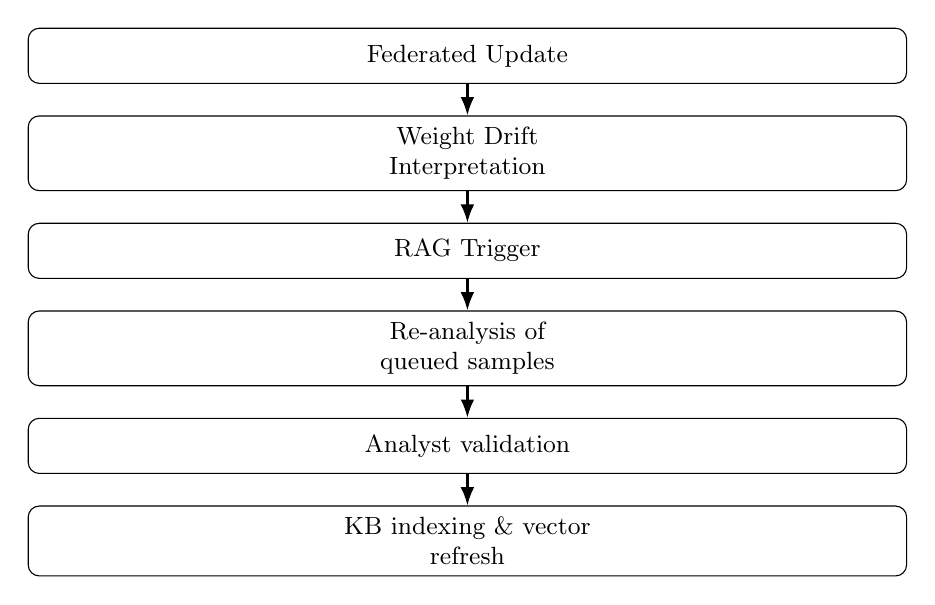
\begin{tikzpicture}[
  font=\small,
  node distance=4mm,
  fbox/.style={draw, rounded corners, align=center, minimum height=7mm, minimum width=0.92\columnwidth, inner sep=4pt},
  farr/.style={-Latex, thick}
]
  \node[fbox] (u) {Federated Update};
  \node[fbox, below=of u] (d) {Weight Drift\\Interpretation};
  \node[fbox, below=of d] (t) {RAG Trigger};
  \node[fbox, below=of t] (r) {Re-analysis of\\queued samples};
  \node[fbox, below=of r] (a) {Analyst validation};
  \node[fbox, below=of a] (k) {KB indexing \& vector\\refresh};

  \draw[farr] (u) -- (d);
  \draw[farr] (d) -- (t);
  \draw[farr] (t) -- (r);
  \draw[farr] (r) -- (a);
  \draw[farr] (a) -- (k);
\end{tikzpicture}
\caption{Federated Learning--RAG bridge workflow: federated updates are interpreted for drift and can trigger retrieval refresh and re-analysis for analyst-facing decisions.}
\label{fig:fed_rag_workflow}
\end{figure}

\begin{figure*}[t]
\centering
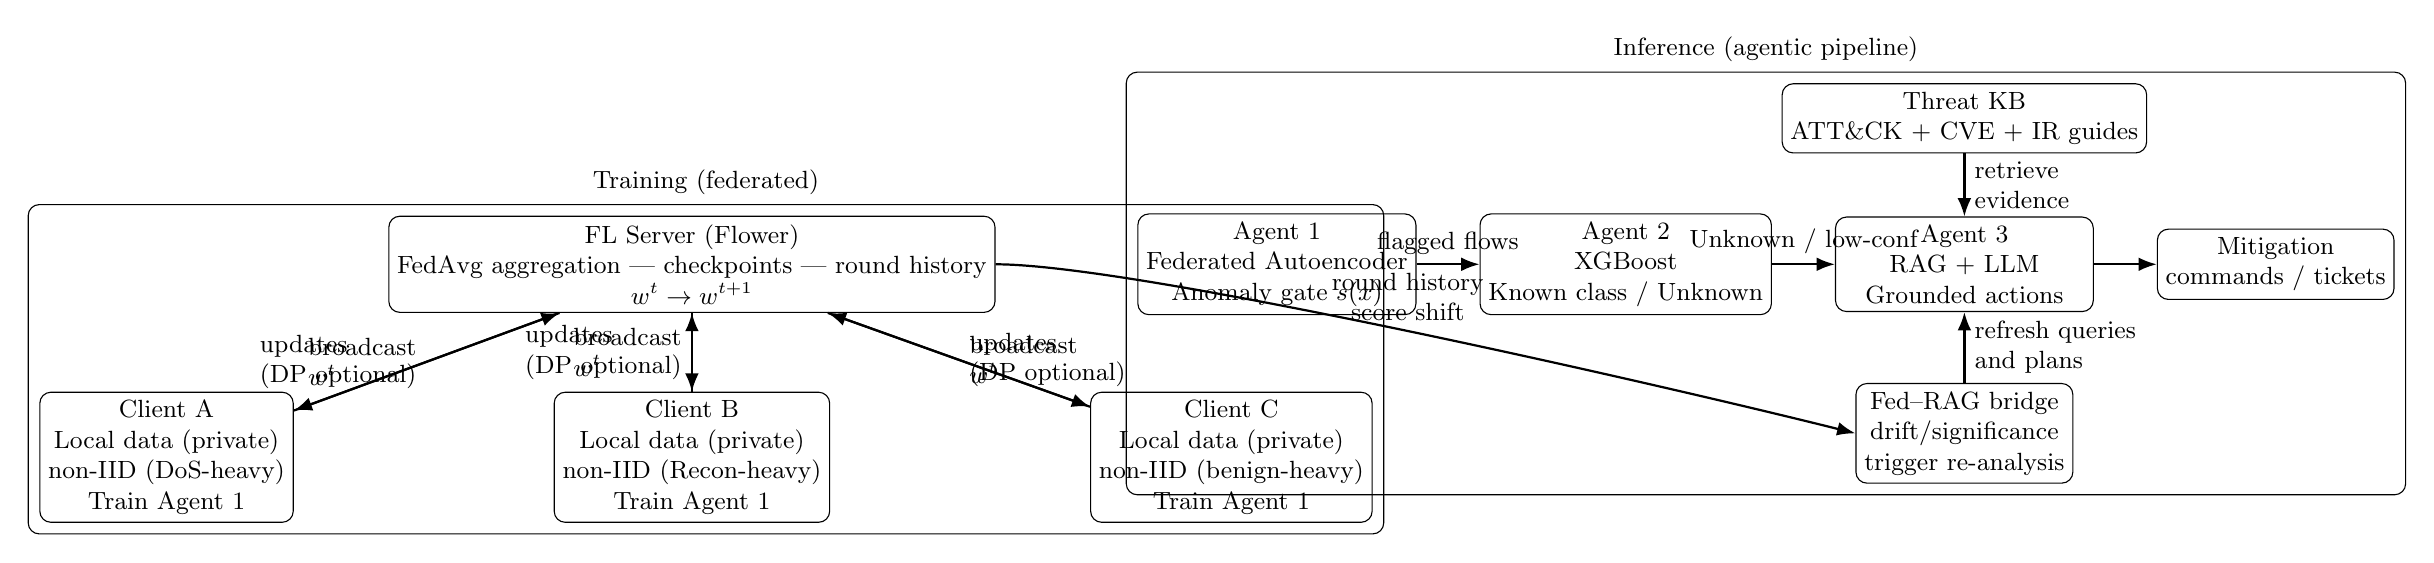
\begin{tikzpicture}[
  font=\small,
  node distance=7mm and 9mm,
  box/.style={draw, rounded corners, align=center, minimum height=7mm, inner sep=3pt},
  bigbox/.style={box, minimum width=0.27\textwidth},
  sbox/.style={box, minimum width=0.19\textwidth},
  arr/.style={-Latex, thick}
]

% --- Training side (FL) ---
\node[box, minimum width=0.27\textwidth] (flsrv) {FL Server (Flower)\\FedAvg aggregation | checkpoints | round history\\$w^{t}\rightarrow w^{t+1}$};
\node[sbox, below left=10mm and 12mm of flsrv] (c1) {Client A\\Local data (private)\\non-IID (DoS-heavy)\\Train Agent 1};
\node[sbox, below=10mm of flsrv] (c2) {Client B\\Local data (private)\\non-IID (Recon-heavy)\\Train Agent 1};
\node[sbox, below right=10mm and 12mm of flsrv] (c3) {Client C\\Local data (private)\\non-IID (benign-heavy)\\Train Agent 1};

\draw[arr] (flsrv) -- node[left, align=left] {broadcast\\$w^t$} (c1);
\draw[arr] (flsrv) -- node[left, align=left] {broadcast\\$w^t$} (c2);
\draw[arr] (flsrv) -- node[right, align=left] {broadcast\\$w^t$} (c3);

\draw[arr] (c1) -- node[left, align=left] {updates\\(DP optional)} (flsrv);
\draw[arr] (c2) -- node[left, align=left] {updates\\(DP optional)} (flsrv);
\draw[arr] (c3) -- node[right, align=left] {updates\\(DP optional)} (flsrv);

% --- Inference side (pipeline) ---
\node[bigbox, right=18mm of flsrv] (a1) {Agent 1\\Federated Autoencoder\\Anomaly gate $s(x)$};
\node[bigbox, right=8mm of a1] (a2) {Agent 2\\XGBoost\\Known class / Unknown};
\node[bigbox, right=8mm of a2] (a3) {Agent 3\\RAG + LLM\\Grounded actions};
\node[box, right=8mm of a3, minimum width=0.18\textwidth] (mit) {Mitigation\\commands / tickets};

\node[box, above=8mm of a3, minimum width=0.22\textwidth] (kb) {Threat KB\\ATT\&CK + CVE + IR guides};

\draw[arr] (a1) -- node[above] {flagged flows} (a2);
\draw[arr] (a2) -- node[above] {Unknown / low-conf} (a3);
\draw[arr] (a3) -- (mit);
\draw[arr] (kb) -- node[right, align=left] {retrieve\\evidence} (a3);

% --- Bridge ---
\node[box, below=9mm of a3, minimum width=0.22\textwidth] (bridge) {Fed--RAG bridge\\drift/significance\\trigger re-analysis};
\draw[arr] (flsrv.east) .. controls +(18mm,0mm) and +(-24mm,6mm) .. node[above, align=center] {round history\\score shift} (bridge.west);
\draw[arr] (bridge.north) -- node[right, align=left] {refresh queries\\and plans} (a3.south);

\node[fit=(flsrv)(c1)(c2)(c3), draw, rounded corners, inner sep=4pt, label={[font=\small]above:Training (federated)}] {};
\node[fit=(a1)(a2)(a3)(kb)(bridge)(mit), draw, rounded corners, inner sep=4pt, label={[font=\small]above:Inference (agentic pipeline)}] {};

\end{tikzpicture}
\caption{Overall system architecture: federated training for Agent~1 only, hierarchical inference across three agents, and a Fed--RAG bridge that refreshes retrieval and explanations when the anomaly profile drifts.}
\label{fig:overall_architecture}
\end{figure*}


\begin{figure}[t]
\centering
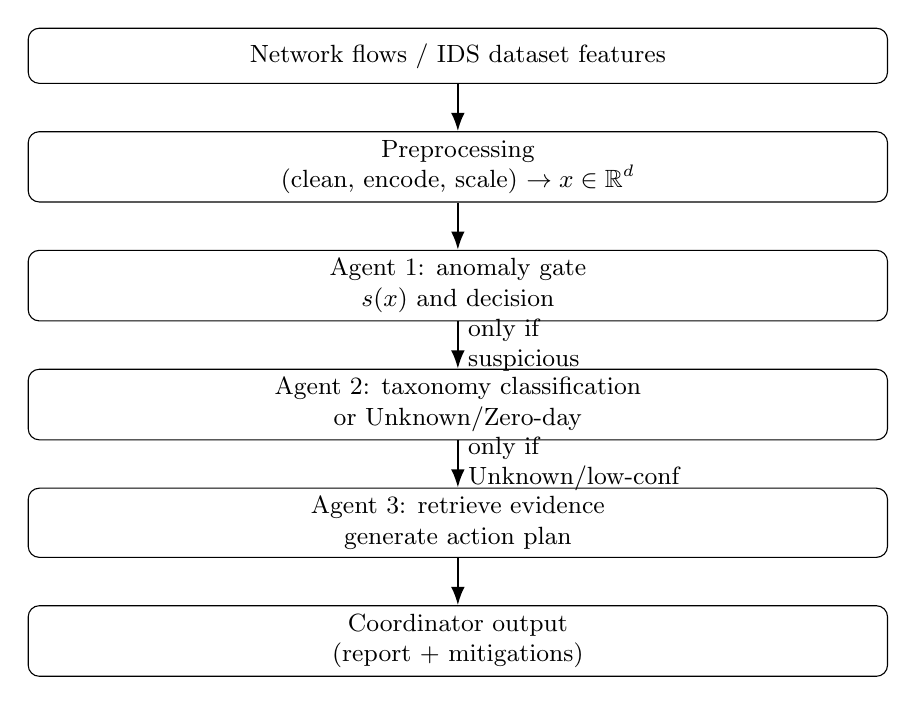
\begin{tikzpicture}[
  font=\small,
  node distance=6mm and 7mm,
  box/.style={draw, rounded corners, align=center, minimum height=7mm, inner sep=3pt, minimum width=0.9\columnwidth},
  arr/.style={-Latex, thick}
]
\node[box] (data) {Network flows / IDS dataset features};
\node[box, below=of data] (prep) {Preprocessing\\(clean, encode, scale) $\rightarrow x\in\mathbb{R}^d$};
\node[box, below=of prep] (g1) {Agent 1: anomaly gate\\$s(x)$ and decision};
\node[box, below=of g1] (g2) {Agent 2: taxonomy classification\\or Unknown/Zero-day};
\node[box, below=of g2] (g3) {Agent 3: retrieve evidence\\generate action plan};
\node[box, below=of g3] (out) {Coordinator output\\(report + mitigations)};

\draw[arr] (data) -- (prep);
\draw[arr] (prep) -- (g1);
\draw[arr] (g1) -- node[right, align=left] {only if\\suspicious} (g2);
\draw[arr] (g2) -- node[right, align=left] {only if\\Unknown/low-conf} (g3);
\draw[arr] (g3) -- (out);
\end{tikzpicture}
\caption{Inference-time dataflow and selective escalation across agents.}
\label{fig:dataflow}
\end{figure}

% Methodology (copy-paste ready)
% Intended usage: % Methodology (copy-paste ready)
% Intended usage: % Methodology (copy-paste ready)
% Intended usage: % Methodology (copy-paste ready)
% Intended usage: \input{methodology_three_agents.tex} from an IEEEtran main paper.
% Required packages in main preamble: amsmath, amssymb, graphicx, booktabs, siunitx, tikz.
% TikZ libraries recommended: \usetikzlibrary{positioning,arrows.meta}
% If you compile standalone, wrap this in an IEEEtran document and include the bibliography.

\section{Methodology}
\label{sec:methodology}

We propose a hierarchical, three-agent intrusion detection and response pipeline that balances (i) real-time filtering, (ii) accurate attack-family classification, and (iii) grounded analyst-facing action planning. The design follows a progressive offloading strategy: low-cost models handle the full traffic stream, while expensive reasoning is invoked only for ambiguous or high-risk events. This is aligned with practical intrusion detection deployments, where early-stage filters reduce throughput to downstream analysis stages \cite{Mirsky2018Kitsune}.

\subsection{Data Preparation and Preprocessing}
\label{sec:data_preparation}

This section describes dataset selection, splits, cleaning, feature engineering, and preprocessing. These steps precede the three agents and ensure that all models operate on consistent feature representations.

\subsubsection{Dataset selection and files}
\textbf{Primary benchmark.} We use UNSW-NB15 as the main benchmark dataset for network intrusion detection, due to its diversity of attack types and its structured feature representation \cite{Moustafa2015UNSW,Moustafa2015UNSW2}.

\textbf{Structured train/test splits.} We use the official structured CSV files:
\begin{itemize}
  \item \emph{Training:} \texttt{UNSW\_NB15\_training-set.csv}
  \item \emph{Testing:} \texttt{UNSW\_NB15\_testing-set.csv}
\end{itemize}

\textbf{Raw distribution evaluation.} To approximate ``in-the-wild'' distributions and validate robustness, we additionally evaluate on the raw UNSW-NB15 split files (\texttt{UNSW-NB15\_1.csv} to \texttt{UNSW-NB15\_4.csv}). These files contain the same 49 columns but do not include headers and may differ in column ordering; therefore we load them with an explicit schema to avoid column-mismatch errors.

\subsubsection{Loading, schema alignment, and cleaning}
We implement dataset ingestion using modular components (a \emph{DataLoader} for loading/initial cleaning and a \emph{Preprocessor} for normalization and encoding). This modularity supports reproducibility and simplifies extending to additional datasets.

\textbf{Schema alignment for raw files.} For raw files without headers, we use a dedicated loader that assigns the 49 column names explicitly (47 features plus \texttt{attack\_cat} and \texttt{label}) and normalizes label fields:
\begin{itemize}
  \item Missing or empty \texttt{attack\_cat} values are mapped to \emph{Normal}.
  \item The binary \texttt{label} field is coerced to integer, where 0 indicates normal and 1 indicates attack.
  \item Category strings are stripped and standardized (e.g., minor whitespace variants are normalized).
\end{itemize}

\textbf{Missing values and numeric coercion.} We treat missing values and invalid numeric fields using robust conversions (coerce-to-numeric followed by imputation). In the general preprocessing pipeline, we use simple imputers (median for numeric features and mode for categorical features) to avoid dropping flows and to preserve deployment realism \cite{Pedregosa2011Scikit}.

\subsubsection{Feature engineering}
We compute derived features that improve separability and capture traffic dynamics. In particular, we compute the connection rate:
\begin{equation}
\texttt{rate} = \frac{\texttt{spkts}+\texttt{dpkts}}{\texttt{dur}+\epsilon},
\end{equation}
with $\epsilon>0$ to avoid division by zero. All engineered features are computed deterministically and are included consistently across train/test and raw evaluation.

\subsubsection{Normalization and encoding}
\textbf{Numerical scaling.} We apply min--max scaling to numerical features, matching the default configuration used by the pipeline. Min--max scaling is particularly suitable for autoencoders, where feature ranges can dominate reconstruction loss if left unnormalized. Our implementation uses standard preprocessing utilities (e.g., \texttt{MinMaxScaler}) \cite{Pedregosa2011Scikit}.

\textbf{Categorical encoding.} Categorical columns (e.g., \texttt{proto}, \texttt{service}, \texttt{state}) are encoded either via integer factorization (label encoding) or via one-hot encoding depending on the experiment configuration. In our baseline, we use label encoding to keep the feature dimensionality stable and to simplify deployment.

\subsubsection{Sampling and reproducibility}
To enable fair comparisons across models, we use fixed random seeds (e.g., \texttt{random\_state}=42) for sampling and train/test splits. All preprocessing artifacts (scaler parameters, encoders, and imputers) are fit on the training split and reused unchanged for validation/test transformations, preventing leakage.

\textbf{Class-imbalance handling for supervised training.} UNSW-NB15 exhibits class imbalance (normal traffic dominates, while some attack categories are rare). For Agent~2 training, we apply SMOTE oversampling \emph{only on the training split} after preprocessing to improve minority-class recall while keeping evaluation unbiased \cite{Chawla2002SMOTE}.

\subsection{Pipeline Overview and Decision Flow}
\label{sec:method_overview}

Let $x \in \mathbb{R}^d$ denote a network-flow feature vector extracted from raw packets (e.g., connection statistics, byte/packet counts, TTL/state features, and aggregate temporal features). We follow the feature format provided by standard IDS benchmarks such as UNSW-NB15 \cite{Moustafa2015UNSW}.

The pipeline produces:
\begin{itemize}
  \item a gate decision (Normal vs Anomalous),
  \item a threat category label among known classes, optionally with an ``Unknown/Zero-day'' flag,
  \item a grounded, structured action plan (recommended actions, relevant ATT\&CK techniques, and candidate CVEs when applicable).
\end{itemize}

\textbf{Preprocessing.} For Agents 1 and 2, tabular features are standardized using statistics computed on the training split (mean/variance scaling). Categorical features (if present) are one-hot encoded. The anomaly score produced by Agent 1 is appended to the Agent 2 feature vector to provide a consistent signal of ``distance from normality''.

\textbf{Hierarchical offloading policy.} The system executes:
\begin{enumerate}
  \item \textbf{Agent 1 (Autoencoder gate):} compute anomaly score $s(x)$ and decide $g(x)\in\{\text{Normal},\text{Anomalous}\}$.
  \item \textbf{Agent 2 (XGBoost classifier):} if $g(x)=\text{Anomalous}$, predict class probabilities $p(y\mid x)$ over $K$ known categories and a confidence score $c(x)=\max_y p(y\mid x)$.
  \item \textbf{Agent 3 (RAG+LLM action planner):} if $c(x)<\gamma$ (low confidence) or if Agent 2 explicitly flags ``Unknown/Zero-day'', retrieve threat-intelligence context and generate an action plan.
\end{enumerate}

\textbf{Rationale.} Agent 1 is optimized for high recall and low latency, ensuring that potentially malicious traffic is not missed. Agent 2 provides a low-cost categorical interpretation to support automated response policies for known threats. Agent 3 is invoked selectively to (i) explain uncertain events and (ii) provide grounded response actions using external threat intelligence, reducing hallucinations relative to purely parametric generation \cite{Lewis2020RAG}.

\begin{figure}[t]
\centering
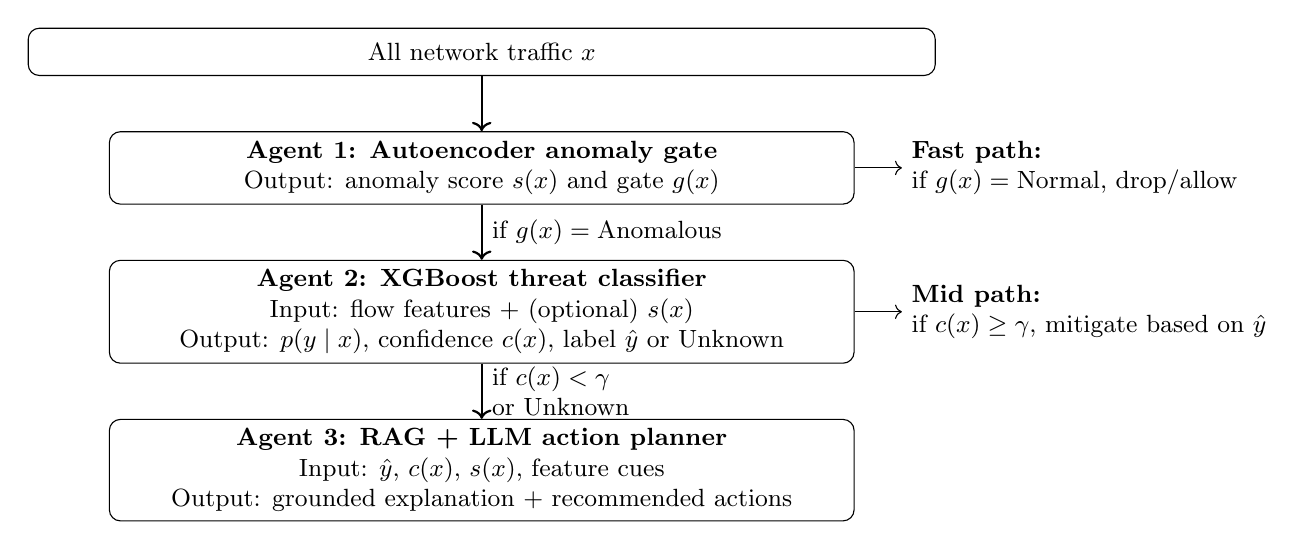
\begin{tikzpicture}[node distance=7mm, font=\small]
  \node[draw, rounded corners, align=center, minimum width=0.95\columnwidth, minimum height=6mm] (traffic) {All network traffic $x$};

  \node[draw, rounded corners, align=center, below=of traffic, minimum width=0.78\columnwidth] (a1) {\textbf{Agent 1: Autoencoder anomaly gate}\\
  Output: anomaly score $s(x)$ and gate $g(x)$};

  \node[draw, rounded corners, align=center, below=of a1, minimum width=0.78\columnwidth] (a2) {\textbf{Agent 2: XGBoost threat classifier}\\
  Input: flow features + (optional) $s(x)$\\
  Output: $p(y\mid x)$, confidence $c(x)$, label $\hat{y}$ or Unknown};

  \node[draw, rounded corners, align=center, below=of a2, minimum width=0.78\columnwidth] (a3) {\textbf{Agent 3: RAG + LLM action planner}\\
  Input: $\hat{y}$, $c(x)$, $s(x)$, feature cues\\
  Output: grounded explanation + recommended actions};

  \draw[->, thick] (traffic) -- (a1);
  \draw[->, thick] (a1) -- node[right, align=left] {if $g(x)=\text{Anomalous}$} (a2);
  \draw[->, thick] (a2) -- node[right, align=left] {if $c(x)<\gamma$\\or Unknown} (a3);

  \node[align=left, right=6mm of a1] (drop) {\textbf{Fast path:}\\if $g(x)=\text{Normal}$, drop/allow};
  \draw[->] (a1.east) -- (drop.west);

  \node[align=left, right=6mm of a2] (mit) {\textbf{Mid path:}\\if $c(x)\ge\gamma$, mitigate based on $\hat{y}$};
  \draw[->] (a2.east) -- (mit.west);
\end{tikzpicture}
\caption{Hierarchical offloading decision flow for the three-agent pipeline.}
\label{fig:hierarchical_offloading}
\end{figure}

\subsection{Agent 1: Autoencoder Anomaly Detector (Gate)}
\label{sec:agent1_method}

\subsubsection{Model architecture}
Agent 1 is a feed-forward PyTorch autoencoder trained to reconstruct benign-dominant traffic. The architecture follows a symmetric bottleneck design (input dimension $d=40$):
\begin{equation}
40 \rightarrow 32 \rightarrow 16 \rightarrow 8 \rightarrow 16 \rightarrow 32 \rightarrow 40,
\end{equation}
where the bottleneck encourages compression into a low-dimensional latent representation. Autoencoders are widely used for anomaly detection by learning normal patterns and flagging reconstruction deviations \cite{Hinton2006Reducing,Mirsky2018Kitsune}.

\textbf{Training objective.} The autoencoder is trained to minimize reconstruction loss on the training split, dominated by Normal traffic:
\begin{equation}
 \min_\theta\; \mathbb{E}_{x\sim\mathcal{D}_{\text{train}}}\left[\lVert x - f_\theta(x)\rVert_2^2\right].
\end{equation}
We use mini-batch optimization (Adam) with early stopping based on validation loss to prevent overfitting.

\subsubsection{Anomaly scoring}
Let $f_\theta(\cdot)$ denote the autoencoder reconstruction function. The anomaly score is computed as the mean squared reconstruction error:
\begin{equation}
 s(x) = \frac{1}{d}\lVert x - f_\theta(x) \rVert_2^2.
\end{equation}
The gate decision is:
\begin{equation}
 g(x) = \mathbb{I}[s(x) \ge \tau],
\end{equation}
where $\tau$ is calibrated on a validation split to achieve a target recall/false-positive trade-off. We select $\tau$ using either (i) a quantile rule on Normal reconstruction errors or (ii) a validation sweep to maximize attack recall at an acceptable false-positive rate.

\textbf{Operating point.} Since the system is designed to avoid missing attacks, we bias $\tau$ toward high recall even if it increases false positives; downstream agents and RAG-based reasoning mitigate the cost by handling only escalated flows.

\subsubsection{Confidence signal}
We additionally expose a normalized confidence proxy derived from the distance to the threshold:
\begin{equation}
 \kappa(x) = \sigma\left(\alpha\,(s(x)-\tau)\right),
\end{equation}
where $\sigma$ is a logistic function and $\alpha$ controls steepness. This scalar is used (i) as an auxiliary feature for Agent 2 to improve separability and (ii) as an escalation cue to Agent 3 when confidence is low.

\subsection{Agent 2: XGBoost Threat Classifier}
\label{sec:agent2_method}

Agent 2 performs supervised multi-class classification over $K=10$ categories (Normal plus nine attack families). We use gradient-boosted decision trees due to their strong performance on tabular intrusion datasets and low inference latency \cite{Chen2016XGBoost}.

\subsubsection{Input features}
For flows flagged anomalous by Agent 1, Agent 2 receives:
\begin{itemize}
  \item raw flow features $x$,
  \item the anomaly score $s(x)$ (or confidence proxy $\kappa(x)$) from Agent 1,
  \item optional engineered statistics (e.g., z-scored feature groups).
\end{itemize}

\textbf{Feature fusion.} The anomaly score acts as a global indicator of deviation from normal behavior and is particularly useful for borderline cases that may be underrepresented in supervised labels.

\subsubsection{Training and imbalance handling}
Class imbalance is addressed using SMOTE oversampling and class-weighted learning, augmented by per-class decision thresholds to balance recall for rare categories \cite{Chawla2002SMOTE}.

Concretely, SMOTE synthesizes minority samples by interpolating between nearest neighbors in feature space. In addition, we apply class weights inversely proportional to class frequency in the loss, and tune per-class decision thresholds on the validation split to improve minority recall without collapsing precision.

We use the following representative hyperparameters (as configured in our implementation): maximum depth $8$, learning rate $0.05$, and $200$ estimators. Early stopping is applied using a validation split.

\subsubsection{Open-set / ``Unknown'' handling (zero-day flag)}
To operationalize zero-day uncertainty, we convert the closed-set classifier into an open-set detector by thresholding confidence:
\begin{equation}
 c(x) = \max_{y\in\{1,\dots,K\}} p(y\mid x).
\end{equation}
If $c(x) < \gamma$ (with $\gamma=0.5$ in our implementation), Agent 2 outputs \emph{Unknown/Zero-day}. This confidence-threshold heuristic is a pragmatic approximation to open-set recognition when explicit unknown-class training is not available; it complements established open-set formulations by explicitly routing uncertain cases to deeper analysis \cite{Scheirer2013OpenSet,Bendale2016OpenMax}.

\textbf{Calibration note.} While boosting models often provide sharp probabilities, confidence thresholds are still sensitive to dataset shift. Therefore, $\gamma$ should be tuned with LOAO-style splits and monitored via false-unknown rate on benign traffic.

\subsection{Agent 3: Retrieval-Augmented Action Planning (RAG+LLM)}
\label{sec:agent3_method}

Agent 3 is invoked only for low-confidence or unknown cases and generates grounded analyst-facing outputs. We adopt Retrieval-Augmented Generation (RAG) to combine parametric LLM reasoning with non-parametric retrieval from a curated knowledge base \cite{Lewis2020RAG}.

\subsubsection{Knowledge sources and representation}
The knowledge base (KB) contains threat intelligence artifacts such as:
\begin{itemize}
  \item MITRE ATT\&CK techniques, tactics, and mitigations \cite{MITREATTACK},
  \item CVE/NVD vulnerability summaries and common exploitation patterns \cite{MITRECVE,NISTNVD},
  \item dataset-specific attack-pattern notes (e.g., UNSW-NB15 and CIC-IDS2017 mappings) \cite{Moustafa2015UNSW,Sharafaldin2018CICIDS}.
\end{itemize}
Each document is embedded into a dense vector space using a sentence embedding model (HuggingFace-style encoders). In our implementation, we use a lightweight sentence-transformer family model to balance retrieval quality and throughput \cite{Reimers2019SentenceBERT}.

\subsubsection{Vector database and retrieval}
We store embeddings in a FAISS vector index for approximate nearest-neighbor retrieval \cite{Johnson2019FAISS}. For a query $q$, the retriever returns top-$k$ documents:
\begin{equation}
 \{d_1,\dots,d_k\} = \operatorname{TopK}(\operatorname{sim}(\phi(q),\phi(d)))
\end{equation}
where $\phi(\cdot)$ maps text to embeddings and $\operatorname{sim}$ is cosine similarity.

\textbf{Retrieval configuration.} We use $k\in\{3,5\}$ depending on prompt budget. Retrieved documents are de-duplicated by (technique ID, CVE ID) to reduce redundancy.

\subsubsection{Retrieval query construction}
The retrieval query is formed from the model outputs and salient feature cues:
\begin{equation}
 q = \{\hat{y},\,c(x),\,s(x),\,\text{feature importance/profile},\,\text{zero-day flag},\,\text{historical scope}\}.
\end{equation}
This structured query is realized as a text prompt that guides the retriever toward relevant technique and vulnerability entries.

\textbf{Why include features?} For ambiguous cases, adding a brief ``feature profile'' (e.g., unusually high packet rate, many half-open connections, abnormal TTL patterns) encourages retrieval of more specific techniques and mitigations, improving actionability.

\subsubsection{Augmentation and generation}
Retrieved evidence is concatenated (with metadata such as technique IDs and severity) and provided to the LLM with instructions to output:
\begin{enumerate}
  \item a concise threat summary,
  \item a ``why novel'' explanation when flagged unknown,
  \item a prioritized \textbf{Recommended Actions} list.
\end{enumerate}
We enforce a structured output format to improve downstream parsing and to support operational use. When the LLM is unavailable, we fall back to deterministic rule-based actions derived from the mapped action space (Table~\ref{tab:action_space}).

\begin{figure}[t]
\centering
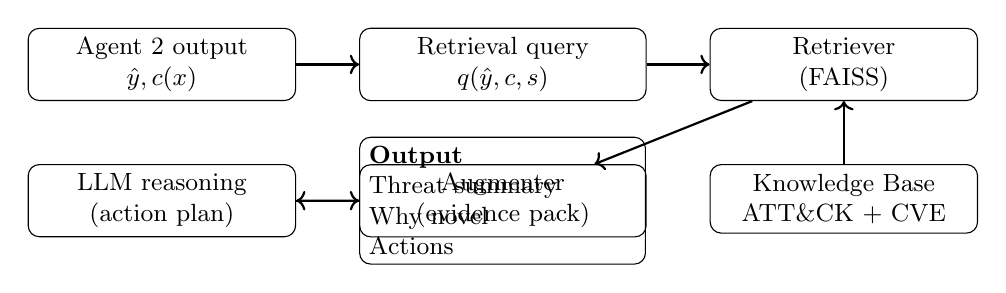
\begin{tikzpicture}[font=\small]
  \node[draw, rounded corners, align=center, minimum width=0.28\columnwidth, minimum height=7mm] (a2out) {Agent 2 output\\$\hat{y}, c(x)$};
  \node[draw, rounded corners, align=center, right=8mm of a2out, minimum width=0.30\columnwidth, minimum height=7mm] (query) {Retrieval query\\$q(\hat{y},c,s)$};
  \node[draw, rounded corners, align=center, right=8mm of query, minimum width=0.28\columnwidth, minimum height=7mm] (retr) {Retriever\\(FAISS)};

  \node[draw, rounded corners, align=center, below=8mm of retr, minimum width=0.28\columnwidth, minimum height=7mm] (kb) {Knowledge Base\\ATT\&CK + CVE};
  \node[draw, rounded corners, align=center, below=8mm of query, minimum width=0.30\columnwidth, minimum height=7mm] (aug) {Augmenter\\(evidence pack)};
  \node[draw, rounded corners, align=center, below=8mm of a2out, minimum width=0.28\columnwidth, minimum height=7mm] (llm) {LLM reasoning\\(action plan)};

  \draw[->, thick] (a2out) -- (query);
  \draw[->, thick] (query) -- (retr);
  \draw[->, thick] (kb) -- (retr);
  \draw[->, thick] (retr) -- (aug);
  \draw[->, thick] (aug) -- (llm);

  \node[draw, rounded corners, align=left, right=8mm of llm, text width=0.28\columnwidth] (out) {\textbf{Output}\\Threat summary\\Why novel\\Actions};
  \draw[->, thick] (llm) -- (out);
\end{tikzpicture}
\caption{Agent 3 RAG pipeline: retrieve evidence then generate structured actions.}
\label{fig:rag_pipeline}
\end{figure}

\subsection{Action Space and Mitigation Mapping}
\label{sec:action_space}

To connect classification outcomes to actionable guidance, we define a compact action space aligned to common NIDS categories and ATT\&CK technique identifiers. The mapping serves two purposes: (i) it provides a consistent schema to evaluate action-plan quality, and (ii) it enables deterministic fallbacks when the LLM cannot be used.

\begin{table}[t]
\caption{Action space mapping from dataset labels to ATT\&CK techniques (representative).}
\label{tab:action_space}
\centering
\begin{tabular}{clll}
\toprule
\textbf{ID} & \textbf{Category} & \textbf{Dataset mapping} & \textbf{MITRE techniques}\\
\midrule
0 & Normal & Normal/Benign & --\\
1 & DoS/DDoS & DoS (UNSW), DoS Hulk (CIC) & T1498, T1499\\
2 & Reconnaissance & Recon (UNSW), PortScan (CIC) & T1046, T1595\\
3 & Exploits & Exploits/Shellcode (UNSW) & T1190, T1059\\
4 & Brute Force & Fuzzers (UNSW) & T1110, T1078\\
5 & Malware & Backdoor/Worms/Generic (UNSW) & T1059, T1071\\
6 & Analysis & Analysis (UNSW), Heartbleed (CIC) & T1040, T1557\\
\bottomrule
\end{tabular}
\end{table}

\subsection{Reproducibility Notes}
\label{sec:reproducibility_notes}

We report all hyperparameters required to reproduce the pipeline, including Agent 1 architecture and $\tau$, Agent 2 hyperparameters and confidence threshold $\gamma$, and Agent 3 retrieval configuration (embedding model, $k$, and KB sources). Since Agent 3 depends on an external LLM endpoint, we fix the prompt template and decoding parameters (temperature, max tokens) and cache retrieved evidence to ensure consistent outputs across reruns. We also log seeds and software versions to reduce variance in reported results \cite{Dodge2019Reporting}.

% -----------------------------
% References for this standalone Methodology section.
% If your main paper uses BibTeX, move these \bibitem entries into your .bib.
\begin{thebibliography}{99}
\bibitem{Moustafa2015UNSW}
N. Moustafa and J. Slay, ``UNSW-NB15: A comprehensive data set for network intrusion detection systems,'' in \emph{Proc. Military Communications and Information Systems Conference (MilCIS)}, 2015.

\bibitem{Moustafa2015UNSW2}
N. Moustafa and J. Slay, ``The evaluation of network anomaly detection systems: Statistical analysis of the UNSW-NB15 data set and the comparison with the KDD99 data set,'' \emph{Information Security Journal: A Global Perspective}, vol. 25, no. 1--3, pp. 18--31, 2016.

\bibitem{Sharafaldin2018CICIDS}
I. Sharafaldin, A. H. Lashkari, and A. A. Ghorbani, ``Toward generating a new intrusion detection dataset and intrusion traffic characterization,'' in \emph{Proc. Int. Conf. Information Systems Security and Privacy (ICISSP)}, 2018.

\bibitem{Hinton2006Reducing}
G. E. Hinton and R. R. Salakhutdinov, ``Reducing the dimensionality of data with neural networks,'' \emph{Science}, vol. 313, no. 5786, pp. 504--507, 2006.

\bibitem{Mirsky2018Kitsune}
Y. Mirsky, T. Doitshman, Y. Elovici, and A. Shabtai, ``Kitsune: An ensemble of autoencoders for online network intrusion detection,'' in \emph{Proc. NDSS}, 2018.

\bibitem{Chen2016XGBoost}
T. Chen and C. Guestrin, ``XGBoost: A scalable tree boosting system,'' in \emph{Proc. ACM SIGKDD}, 2016, pp. 785--794.

\bibitem{Chawla2002SMOTE}
N. V. Chawla, K. W. Bowyer, L. O. Hall, and W. P. Kegelmeyer, ``SMOTE: Synthetic minority over-sampling technique,'' \emph{J. Artif. Intell. Res.}, vol. 16, pp. 321--357, 2002.

\bibitem{Pedregosa2011Scikit}
F. Pedregosa \emph{et al.}, ``Scikit-learn: Machine learning in Python,'' \emph{J. Mach. Learn. Res.}, vol. 12, pp. 2825--2830, 2011.

\bibitem{Scheirer2013OpenSet}
W. J. Scheirer, A. Rocha, R. J. Micheals, and T. E. Boult, ``Toward open set recognition,'' \emph{IEEE Trans. Pattern Anal. Mach. Intell.}, vol. 35, no. 7, pp. 1757--1772, 2013.

\bibitem{Bendale2016OpenMax}
A. Bendale and T. E. Boult, ``Towards open set deep networks,'' in \emph{Proc. CVPR}, 2016.

\bibitem{Lewis2020RAG}
P. Lewis \emph{et al.}, ``Retrieval-augmented generation for knowledge-intensive NLP tasks,'' in \emph{Proc. NeurIPS}, 2020.

\bibitem{Reimers2019SentenceBERT}
N. Reimers and I. Gurevych, ``Sentence-BERT: Sentence embeddings using Siamese BERT-networks,'' in \emph{Proc. EMNLP-IJCNLP}, 2019.

\bibitem{Johnson2019FAISS}
J. Johnson, M. Douze, and H. J\'egou, ``Billion-scale similarity search with GPUs,'' \emph{IEEE Trans. Big Data}, vol. 7, no. 3, pp. 535--547, 2021 (early access 2019).

\bibitem{MITREATTACK}
MITRE, ``MITRE ATT\&CK,'' 2026. [Online]. Available: \url{https://attack.mitre.org/}. Accessed: Apr. 18, 2026.

\bibitem{MITRECVE}
MITRE, ``Common Vulnerabilities and Exposures (CVE),'' 2026. [Online]. Available: \url{https://www.cve.org/}. Accessed: Apr. 18, 2026.

\bibitem{NISTNVD}
National Institute of Standards and Technology, ``National Vulnerability Database (NVD),'' 2026. [Online]. Available: \url{https://nvd.nist.gov/}. Accessed: Apr. 18, 2026.

\bibitem{Dodge2019Reporting}
J. Dodge \emph{et al.}, ``Show your work: Improved reporting of experimental results,'' in \emph{Proc. EMNLP-IJCNLP}, 2019.
\end{thebibliography}
 from an IEEEtran main paper.
% Required packages in main preamble: amsmath, amssymb, graphicx, booktabs, siunitx, tikz.
% TikZ libraries recommended: \usetikzlibrary{positioning,arrows.meta}
% If you compile standalone, wrap this in an IEEEtran document and include the bibliography.

\section{Methodology}
\label{sec:methodology}

We propose a hierarchical, three-agent intrusion detection and response pipeline that balances (i) real-time filtering, (ii) accurate attack-family classification, and (iii) grounded analyst-facing action planning. The design follows a progressive offloading strategy: low-cost models handle the full traffic stream, while expensive reasoning is invoked only for ambiguous or high-risk events. This is aligned with practical intrusion detection deployments, where early-stage filters reduce throughput to downstream analysis stages \cite{Mirsky2018Kitsune}.

\subsection{Data Preparation and Preprocessing}
\label{sec:data_preparation}

This section describes dataset selection, splits, cleaning, feature engineering, and preprocessing. These steps precede the three agents and ensure that all models operate on consistent feature representations.

\subsubsection{Dataset selection and files}
\textbf{Primary benchmark.} We use UNSW-NB15 as the main benchmark dataset for network intrusion detection, due to its diversity of attack types and its structured feature representation \cite{Moustafa2015UNSW,Moustafa2015UNSW2}.

\textbf{Structured train/test splits.} We use the official structured CSV files:
\begin{itemize}
  \item \emph{Training:} \texttt{UNSW\_NB15\_training-set.csv}
  \item \emph{Testing:} \texttt{UNSW\_NB15\_testing-set.csv}
\end{itemize}

\textbf{Raw distribution evaluation.} To approximate ``in-the-wild'' distributions and validate robustness, we additionally evaluate on the raw UNSW-NB15 split files (\texttt{UNSW-NB15\_1.csv} to \texttt{UNSW-NB15\_4.csv}). These files contain the same 49 columns but do not include headers and may differ in column ordering; therefore we load them with an explicit schema to avoid column-mismatch errors.

\subsubsection{Loading, schema alignment, and cleaning}
We implement dataset ingestion using modular components (a \emph{DataLoader} for loading/initial cleaning and a \emph{Preprocessor} for normalization and encoding). This modularity supports reproducibility and simplifies extending to additional datasets.

\textbf{Schema alignment for raw files.} For raw files without headers, we use a dedicated loader that assigns the 49 column names explicitly (47 features plus \texttt{attack\_cat} and \texttt{label}) and normalizes label fields:
\begin{itemize}
  \item Missing or empty \texttt{attack\_cat} values are mapped to \emph{Normal}.
  \item The binary \texttt{label} field is coerced to integer, where 0 indicates normal and 1 indicates attack.
  \item Category strings are stripped and standardized (e.g., minor whitespace variants are normalized).
\end{itemize}

\textbf{Missing values and numeric coercion.} We treat missing values and invalid numeric fields using robust conversions (coerce-to-numeric followed by imputation). In the general preprocessing pipeline, we use simple imputers (median for numeric features and mode for categorical features) to avoid dropping flows and to preserve deployment realism \cite{Pedregosa2011Scikit}.

\subsubsection{Feature engineering}
We compute derived features that improve separability and capture traffic dynamics. In particular, we compute the connection rate:
\begin{equation}
\texttt{rate} = \frac{\texttt{spkts}+\texttt{dpkts}}{\texttt{dur}+\epsilon},
\end{equation}
with $\epsilon>0$ to avoid division by zero. All engineered features are computed deterministically and are included consistently across train/test and raw evaluation.

\subsubsection{Normalization and encoding}
\textbf{Numerical scaling.} We apply min--max scaling to numerical features, matching the default configuration used by the pipeline. Min--max scaling is particularly suitable for autoencoders, where feature ranges can dominate reconstruction loss if left unnormalized. Our implementation uses standard preprocessing utilities (e.g., \texttt{MinMaxScaler}) \cite{Pedregosa2011Scikit}.

\textbf{Categorical encoding.} Categorical columns (e.g., \texttt{proto}, \texttt{service}, \texttt{state}) are encoded either via integer factorization (label encoding) or via one-hot encoding depending on the experiment configuration. In our baseline, we use label encoding to keep the feature dimensionality stable and to simplify deployment.

\subsubsection{Sampling and reproducibility}
To enable fair comparisons across models, we use fixed random seeds (e.g., \texttt{random\_state}=42) for sampling and train/test splits. All preprocessing artifacts (scaler parameters, encoders, and imputers) are fit on the training split and reused unchanged for validation/test transformations, preventing leakage.

\textbf{Class-imbalance handling for supervised training.} UNSW-NB15 exhibits class imbalance (normal traffic dominates, while some attack categories are rare). For Agent~2 training, we apply SMOTE oversampling \emph{only on the training split} after preprocessing to improve minority-class recall while keeping evaluation unbiased \cite{Chawla2002SMOTE}.

\subsection{Pipeline Overview and Decision Flow}
\label{sec:method_overview}

Let $x \in \mathbb{R}^d$ denote a network-flow feature vector extracted from raw packets (e.g., connection statistics, byte/packet counts, TTL/state features, and aggregate temporal features). We follow the feature format provided by standard IDS benchmarks such as UNSW-NB15 \cite{Moustafa2015UNSW}.

The pipeline produces:
\begin{itemize}
  \item a gate decision (Normal vs Anomalous),
  \item a threat category label among known classes, optionally with an ``Unknown/Zero-day'' flag,
  \item a grounded, structured action plan (recommended actions, relevant ATT\&CK techniques, and candidate CVEs when applicable).
\end{itemize}

\textbf{Preprocessing.} For Agents 1 and 2, tabular features are standardized using statistics computed on the training split (mean/variance scaling). Categorical features (if present) are one-hot encoded. The anomaly score produced by Agent 1 is appended to the Agent 2 feature vector to provide a consistent signal of ``distance from normality''.

\textbf{Hierarchical offloading policy.} The system executes:
\begin{enumerate}
  \item \textbf{Agent 1 (Autoencoder gate):} compute anomaly score $s(x)$ and decide $g(x)\in\{\text{Normal},\text{Anomalous}\}$.
  \item \textbf{Agent 2 (XGBoost classifier):} if $g(x)=\text{Anomalous}$, predict class probabilities $p(y\mid x)$ over $K$ known categories and a confidence score $c(x)=\max_y p(y\mid x)$.
  \item \textbf{Agent 3 (RAG+LLM action planner):} if $c(x)<\gamma$ (low confidence) or if Agent 2 explicitly flags ``Unknown/Zero-day'', retrieve threat-intelligence context and generate an action plan.
\end{enumerate}

\textbf{Rationale.} Agent 1 is optimized for high recall and low latency, ensuring that potentially malicious traffic is not missed. Agent 2 provides a low-cost categorical interpretation to support automated response policies for known threats. Agent 3 is invoked selectively to (i) explain uncertain events and (ii) provide grounded response actions using external threat intelligence, reducing hallucinations relative to purely parametric generation \cite{Lewis2020RAG}.

\begin{figure}[t]
\centering
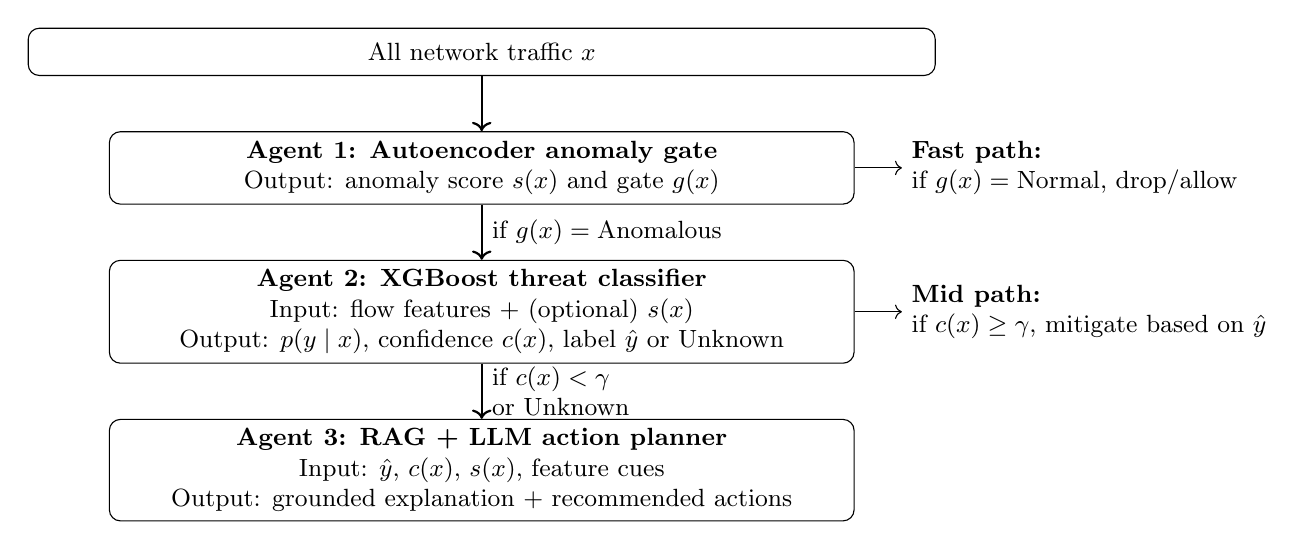
\begin{tikzpicture}[node distance=7mm, font=\small]
  \node[draw, rounded corners, align=center, minimum width=0.95\columnwidth, minimum height=6mm] (traffic) {All network traffic $x$};

  \node[draw, rounded corners, align=center, below=of traffic, minimum width=0.78\columnwidth] (a1) {\textbf{Agent 1: Autoencoder anomaly gate}\\
  Output: anomaly score $s(x)$ and gate $g(x)$};

  \node[draw, rounded corners, align=center, below=of a1, minimum width=0.78\columnwidth] (a2) {\textbf{Agent 2: XGBoost threat classifier}\\
  Input: flow features + (optional) $s(x)$\\
  Output: $p(y\mid x)$, confidence $c(x)$, label $\hat{y}$ or Unknown};

  \node[draw, rounded corners, align=center, below=of a2, minimum width=0.78\columnwidth] (a3) {\textbf{Agent 3: RAG + LLM action planner}\\
  Input: $\hat{y}$, $c(x)$, $s(x)$, feature cues\\
  Output: grounded explanation + recommended actions};

  \draw[->, thick] (traffic) -- (a1);
  \draw[->, thick] (a1) -- node[right, align=left] {if $g(x)=\text{Anomalous}$} (a2);
  \draw[->, thick] (a2) -- node[right, align=left] {if $c(x)<\gamma$\\or Unknown} (a3);

  \node[align=left, right=6mm of a1] (drop) {\textbf{Fast path:}\\if $g(x)=\text{Normal}$, drop/allow};
  \draw[->] (a1.east) -- (drop.west);

  \node[align=left, right=6mm of a2] (mit) {\textbf{Mid path:}\\if $c(x)\ge\gamma$, mitigate based on $\hat{y}$};
  \draw[->] (a2.east) -- (mit.west);
\end{tikzpicture}
\caption{Hierarchical offloading decision flow for the three-agent pipeline.}
\label{fig:hierarchical_offloading}
\end{figure}

\subsection{Agent 1: Autoencoder Anomaly Detector (Gate)}
\label{sec:agent1_method}

\subsubsection{Model architecture}
Agent 1 is a feed-forward PyTorch autoencoder trained to reconstruct benign-dominant traffic. The architecture follows a symmetric bottleneck design (input dimension $d=40$):
\begin{equation}
40 \rightarrow 32 \rightarrow 16 \rightarrow 8 \rightarrow 16 \rightarrow 32 \rightarrow 40,
\end{equation}
where the bottleneck encourages compression into a low-dimensional latent representation. Autoencoders are widely used for anomaly detection by learning normal patterns and flagging reconstruction deviations \cite{Hinton2006Reducing,Mirsky2018Kitsune}.

\textbf{Training objective.} The autoencoder is trained to minimize reconstruction loss on the training split, dominated by Normal traffic:
\begin{equation}
 \min_\theta\; \mathbb{E}_{x\sim\mathcal{D}_{\text{train}}}\left[\lVert x - f_\theta(x)\rVert_2^2\right].
\end{equation}
We use mini-batch optimization (Adam) with early stopping based on validation loss to prevent overfitting.

\subsubsection{Anomaly scoring}
Let $f_\theta(\cdot)$ denote the autoencoder reconstruction function. The anomaly score is computed as the mean squared reconstruction error:
\begin{equation}
 s(x) = \frac{1}{d}\lVert x - f_\theta(x) \rVert_2^2.
\end{equation}
The gate decision is:
\begin{equation}
 g(x) = \mathbb{I}[s(x) \ge \tau],
\end{equation}
where $\tau$ is calibrated on a validation split to achieve a target recall/false-positive trade-off. We select $\tau$ using either (i) a quantile rule on Normal reconstruction errors or (ii) a validation sweep to maximize attack recall at an acceptable false-positive rate.

\textbf{Operating point.} Since the system is designed to avoid missing attacks, we bias $\tau$ toward high recall even if it increases false positives; downstream agents and RAG-based reasoning mitigate the cost by handling only escalated flows.

\subsubsection{Confidence signal}
We additionally expose a normalized confidence proxy derived from the distance to the threshold:
\begin{equation}
 \kappa(x) = \sigma\left(\alpha\,(s(x)-\tau)\right),
\end{equation}
where $\sigma$ is a logistic function and $\alpha$ controls steepness. This scalar is used (i) as an auxiliary feature for Agent 2 to improve separability and (ii) as an escalation cue to Agent 3 when confidence is low.

\subsection{Agent 2: XGBoost Threat Classifier}
\label{sec:agent2_method}

Agent 2 performs supervised multi-class classification over $K=10$ categories (Normal plus nine attack families). We use gradient-boosted decision trees due to their strong performance on tabular intrusion datasets and low inference latency \cite{Chen2016XGBoost}.

\subsubsection{Input features}
For flows flagged anomalous by Agent 1, Agent 2 receives:
\begin{itemize}
  \item raw flow features $x$,
  \item the anomaly score $s(x)$ (or confidence proxy $\kappa(x)$) from Agent 1,
  \item optional engineered statistics (e.g., z-scored feature groups).
\end{itemize}

\textbf{Feature fusion.} The anomaly score acts as a global indicator of deviation from normal behavior and is particularly useful for borderline cases that may be underrepresented in supervised labels.

\subsubsection{Training and imbalance handling}
Class imbalance is addressed using SMOTE oversampling and class-weighted learning, augmented by per-class decision thresholds to balance recall for rare categories \cite{Chawla2002SMOTE}.

Concretely, SMOTE synthesizes minority samples by interpolating between nearest neighbors in feature space. In addition, we apply class weights inversely proportional to class frequency in the loss, and tune per-class decision thresholds on the validation split to improve minority recall without collapsing precision.

We use the following representative hyperparameters (as configured in our implementation): maximum depth $8$, learning rate $0.05$, and $200$ estimators. Early stopping is applied using a validation split.

\subsubsection{Open-set / ``Unknown'' handling (zero-day flag)}
To operationalize zero-day uncertainty, we convert the closed-set classifier into an open-set detector by thresholding confidence:
\begin{equation}
 c(x) = \max_{y\in\{1,\dots,K\}} p(y\mid x).
\end{equation}
If $c(x) < \gamma$ (with $\gamma=0.5$ in our implementation), Agent 2 outputs \emph{Unknown/Zero-day}. This confidence-threshold heuristic is a pragmatic approximation to open-set recognition when explicit unknown-class training is not available; it complements established open-set formulations by explicitly routing uncertain cases to deeper analysis \cite{Scheirer2013OpenSet,Bendale2016OpenMax}.

\textbf{Calibration note.} While boosting models often provide sharp probabilities, confidence thresholds are still sensitive to dataset shift. Therefore, $\gamma$ should be tuned with LOAO-style splits and monitored via false-unknown rate on benign traffic.

\subsection{Agent 3: Retrieval-Augmented Action Planning (RAG+LLM)}
\label{sec:agent3_method}

Agent 3 is invoked only for low-confidence or unknown cases and generates grounded analyst-facing outputs. We adopt Retrieval-Augmented Generation (RAG) to combine parametric LLM reasoning with non-parametric retrieval from a curated knowledge base \cite{Lewis2020RAG}.

\subsubsection{Knowledge sources and representation}
The knowledge base (KB) contains threat intelligence artifacts such as:
\begin{itemize}
  \item MITRE ATT\&CK techniques, tactics, and mitigations \cite{MITREATTACK},
  \item CVE/NVD vulnerability summaries and common exploitation patterns \cite{MITRECVE,NISTNVD},
  \item dataset-specific attack-pattern notes (e.g., UNSW-NB15 and CIC-IDS2017 mappings) \cite{Moustafa2015UNSW,Sharafaldin2018CICIDS}.
\end{itemize}
Each document is embedded into a dense vector space using a sentence embedding model (HuggingFace-style encoders). In our implementation, we use a lightweight sentence-transformer family model to balance retrieval quality and throughput \cite{Reimers2019SentenceBERT}.

\subsubsection{Vector database and retrieval}
We store embeddings in a FAISS vector index for approximate nearest-neighbor retrieval \cite{Johnson2019FAISS}. For a query $q$, the retriever returns top-$k$ documents:
\begin{equation}
 \{d_1,\dots,d_k\} = \operatorname{TopK}(\operatorname{sim}(\phi(q),\phi(d)))
\end{equation}
where $\phi(\cdot)$ maps text to embeddings and $\operatorname{sim}$ is cosine similarity.

\textbf{Retrieval configuration.} We use $k\in\{3,5\}$ depending on prompt budget. Retrieved documents are de-duplicated by (technique ID, CVE ID) to reduce redundancy.

\subsubsection{Retrieval query construction}
The retrieval query is formed from the model outputs and salient feature cues:
\begin{equation}
 q = \{\hat{y},\,c(x),\,s(x),\,\text{feature importance/profile},\,\text{zero-day flag},\,\text{historical scope}\}.
\end{equation}
This structured query is realized as a text prompt that guides the retriever toward relevant technique and vulnerability entries.

\textbf{Why include features?} For ambiguous cases, adding a brief ``feature profile'' (e.g., unusually high packet rate, many half-open connections, abnormal TTL patterns) encourages retrieval of more specific techniques and mitigations, improving actionability.

\subsubsection{Augmentation and generation}
Retrieved evidence is concatenated (with metadata such as technique IDs and severity) and provided to the LLM with instructions to output:
\begin{enumerate}
  \item a concise threat summary,
  \item a ``why novel'' explanation when flagged unknown,
  \item a prioritized \textbf{Recommended Actions} list.
\end{enumerate}
We enforce a structured output format to improve downstream parsing and to support operational use. When the LLM is unavailable, we fall back to deterministic rule-based actions derived from the mapped action space (Table~\ref{tab:action_space}).

\begin{figure}[t]
\centering
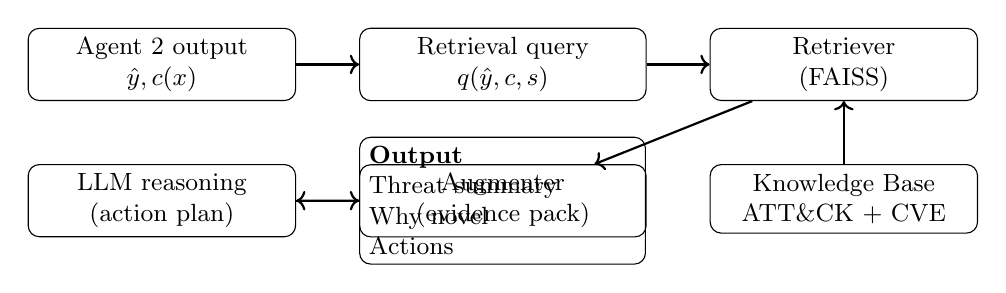
\begin{tikzpicture}[font=\small]
  \node[draw, rounded corners, align=center, minimum width=0.28\columnwidth, minimum height=7mm] (a2out) {Agent 2 output\\$\hat{y}, c(x)$};
  \node[draw, rounded corners, align=center, right=8mm of a2out, minimum width=0.30\columnwidth, minimum height=7mm] (query) {Retrieval query\\$q(\hat{y},c,s)$};
  \node[draw, rounded corners, align=center, right=8mm of query, minimum width=0.28\columnwidth, minimum height=7mm] (retr) {Retriever\\(FAISS)};

  \node[draw, rounded corners, align=center, below=8mm of retr, minimum width=0.28\columnwidth, minimum height=7mm] (kb) {Knowledge Base\\ATT\&CK + CVE};
  \node[draw, rounded corners, align=center, below=8mm of query, minimum width=0.30\columnwidth, minimum height=7mm] (aug) {Augmenter\\(evidence pack)};
  \node[draw, rounded corners, align=center, below=8mm of a2out, minimum width=0.28\columnwidth, minimum height=7mm] (llm) {LLM reasoning\\(action plan)};

  \draw[->, thick] (a2out) -- (query);
  \draw[->, thick] (query) -- (retr);
  \draw[->, thick] (kb) -- (retr);
  \draw[->, thick] (retr) -- (aug);
  \draw[->, thick] (aug) -- (llm);

  \node[draw, rounded corners, align=left, right=8mm of llm, text width=0.28\columnwidth] (out) {\textbf{Output}\\Threat summary\\Why novel\\Actions};
  \draw[->, thick] (llm) -- (out);
\end{tikzpicture}
\caption{Agent 3 RAG pipeline: retrieve evidence then generate structured actions.}
\label{fig:rag_pipeline}
\end{figure}

\subsection{Action Space and Mitigation Mapping}
\label{sec:action_space}

To connect classification outcomes to actionable guidance, we define a compact action space aligned to common NIDS categories and ATT\&CK technique identifiers. The mapping serves two purposes: (i) it provides a consistent schema to evaluate action-plan quality, and (ii) it enables deterministic fallbacks when the LLM cannot be used.

\begin{table}[t]
\caption{Action space mapping from dataset labels to ATT\&CK techniques (representative).}
\label{tab:action_space}
\centering
\begin{tabular}{clll}
\toprule
\textbf{ID} & \textbf{Category} & \textbf{Dataset mapping} & \textbf{MITRE techniques}\\
\midrule
0 & Normal & Normal/Benign & --\\
1 & DoS/DDoS & DoS (UNSW), DoS Hulk (CIC) & T1498, T1499\\
2 & Reconnaissance & Recon (UNSW), PortScan (CIC) & T1046, T1595\\
3 & Exploits & Exploits/Shellcode (UNSW) & T1190, T1059\\
4 & Brute Force & Fuzzers (UNSW) & T1110, T1078\\
5 & Malware & Backdoor/Worms/Generic (UNSW) & T1059, T1071\\
6 & Analysis & Analysis (UNSW), Heartbleed (CIC) & T1040, T1557\\
\bottomrule
\end{tabular}
\end{table}

\subsection{Reproducibility Notes}
\label{sec:reproducibility_notes}

We report all hyperparameters required to reproduce the pipeline, including Agent 1 architecture and $\tau$, Agent 2 hyperparameters and confidence threshold $\gamma$, and Agent 3 retrieval configuration (embedding model, $k$, and KB sources). Since Agent 3 depends on an external LLM endpoint, we fix the prompt template and decoding parameters (temperature, max tokens) and cache retrieved evidence to ensure consistent outputs across reruns. We also log seeds and software versions to reduce variance in reported results \cite{Dodge2019Reporting}.

% -----------------------------
% References for this standalone Methodology section.
% If your main paper uses BibTeX, move these \bibitem entries into your .bib.
\begin{thebibliography}{99}
\bibitem{Moustafa2015UNSW}
N. Moustafa and J. Slay, ``UNSW-NB15: A comprehensive data set for network intrusion detection systems,'' in \emph{Proc. Military Communications and Information Systems Conference (MilCIS)}, 2015.

\bibitem{Moustafa2015UNSW2}
N. Moustafa and J. Slay, ``The evaluation of network anomaly detection systems: Statistical analysis of the UNSW-NB15 data set and the comparison with the KDD99 data set,'' \emph{Information Security Journal: A Global Perspective}, vol. 25, no. 1--3, pp. 18--31, 2016.

\bibitem{Sharafaldin2018CICIDS}
I. Sharafaldin, A. H. Lashkari, and A. A. Ghorbani, ``Toward generating a new intrusion detection dataset and intrusion traffic characterization,'' in \emph{Proc. Int. Conf. Information Systems Security and Privacy (ICISSP)}, 2018.

\bibitem{Hinton2006Reducing}
G. E. Hinton and R. R. Salakhutdinov, ``Reducing the dimensionality of data with neural networks,'' \emph{Science}, vol. 313, no. 5786, pp. 504--507, 2006.

\bibitem{Mirsky2018Kitsune}
Y. Mirsky, T. Doitshman, Y. Elovici, and A. Shabtai, ``Kitsune: An ensemble of autoencoders for online network intrusion detection,'' in \emph{Proc. NDSS}, 2018.

\bibitem{Chen2016XGBoost}
T. Chen and C. Guestrin, ``XGBoost: A scalable tree boosting system,'' in \emph{Proc. ACM SIGKDD}, 2016, pp. 785--794.

\bibitem{Chawla2002SMOTE}
N. V. Chawla, K. W. Bowyer, L. O. Hall, and W. P. Kegelmeyer, ``SMOTE: Synthetic minority over-sampling technique,'' \emph{J. Artif. Intell. Res.}, vol. 16, pp. 321--357, 2002.

\bibitem{Pedregosa2011Scikit}
F. Pedregosa \emph{et al.}, ``Scikit-learn: Machine learning in Python,'' \emph{J. Mach. Learn. Res.}, vol. 12, pp. 2825--2830, 2011.

\bibitem{Scheirer2013OpenSet}
W. J. Scheirer, A. Rocha, R. J. Micheals, and T. E. Boult, ``Toward open set recognition,'' \emph{IEEE Trans. Pattern Anal. Mach. Intell.}, vol. 35, no. 7, pp. 1757--1772, 2013.

\bibitem{Bendale2016OpenMax}
A. Bendale and T. E. Boult, ``Towards open set deep networks,'' in \emph{Proc. CVPR}, 2016.

\bibitem{Lewis2020RAG}
P. Lewis \emph{et al.}, ``Retrieval-augmented generation for knowledge-intensive NLP tasks,'' in \emph{Proc. NeurIPS}, 2020.

\bibitem{Reimers2019SentenceBERT}
N. Reimers and I. Gurevych, ``Sentence-BERT: Sentence embeddings using Siamese BERT-networks,'' in \emph{Proc. EMNLP-IJCNLP}, 2019.

\bibitem{Johnson2019FAISS}
J. Johnson, M. Douze, and H. J\'egou, ``Billion-scale similarity search with GPUs,'' \emph{IEEE Trans. Big Data}, vol. 7, no. 3, pp. 535--547, 2021 (early access 2019).

\bibitem{MITREATTACK}
MITRE, ``MITRE ATT\&CK,'' 2026. [Online]. Available: \url{https://attack.mitre.org/}. Accessed: Apr. 18, 2026.

\bibitem{MITRECVE}
MITRE, ``Common Vulnerabilities and Exposures (CVE),'' 2026. [Online]. Available: \url{https://www.cve.org/}. Accessed: Apr. 18, 2026.

\bibitem{NISTNVD}
National Institute of Standards and Technology, ``National Vulnerability Database (NVD),'' 2026. [Online]. Available: \url{https://nvd.nist.gov/}. Accessed: Apr. 18, 2026.

\bibitem{Dodge2019Reporting}
J. Dodge \emph{et al.}, ``Show your work: Improved reporting of experimental results,'' in \emph{Proc. EMNLP-IJCNLP}, 2019.
\end{thebibliography}
 from an IEEEtran main paper.
% Required packages in main preamble: amsmath, amssymb, graphicx, booktabs, siunitx, tikz.
% TikZ libraries recommended: \usetikzlibrary{positioning,arrows.meta}
% If you compile standalone, wrap this in an IEEEtran document and include the bibliography.

\section{Methodology}
\label{sec:methodology}

We propose a hierarchical, three-agent intrusion detection and response pipeline that balances (i) real-time filtering, (ii) accurate attack-family classification, and (iii) grounded analyst-facing action planning. The design follows a progressive offloading strategy: low-cost models handle the full traffic stream, while expensive reasoning is invoked only for ambiguous or high-risk events. This is aligned with practical intrusion detection deployments, where early-stage filters reduce throughput to downstream analysis stages \cite{Mirsky2018Kitsune}.

\subsection{Data Preparation and Preprocessing}
\label{sec:data_preparation}

This section describes dataset selection, splits, cleaning, feature engineering, and preprocessing. These steps precede the three agents and ensure that all models operate on consistent feature representations.

\subsubsection{Dataset selection and files}
\textbf{Primary benchmark.} We use UNSW-NB15 as the main benchmark dataset for network intrusion detection, due to its diversity of attack types and its structured feature representation \cite{Moustafa2015UNSW,Moustafa2015UNSW2}.

\textbf{Structured train/test splits.} We use the official structured CSV files:
\begin{itemize}
  \item \emph{Training:} \texttt{UNSW\_NB15\_training-set.csv}
  \item \emph{Testing:} \texttt{UNSW\_NB15\_testing-set.csv}
\end{itemize}

\textbf{Raw distribution evaluation.} To approximate ``in-the-wild'' distributions and validate robustness, we additionally evaluate on the raw UNSW-NB15 split files (\texttt{UNSW-NB15\_1.csv} to \texttt{UNSW-NB15\_4.csv}). These files contain the same 49 columns but do not include headers and may differ in column ordering; therefore we load them with an explicit schema to avoid column-mismatch errors.

\subsubsection{Loading, schema alignment, and cleaning}
We implement dataset ingestion using modular components (a \emph{DataLoader} for loading/initial cleaning and a \emph{Preprocessor} for normalization and encoding). This modularity supports reproducibility and simplifies extending to additional datasets.

\textbf{Schema alignment for raw files.} For raw files without headers, we use a dedicated loader that assigns the 49 column names explicitly (47 features plus \texttt{attack\_cat} and \texttt{label}) and normalizes label fields:
\begin{itemize}
  \item Missing or empty \texttt{attack\_cat} values are mapped to \emph{Normal}.
  \item The binary \texttt{label} field is coerced to integer, where 0 indicates normal and 1 indicates attack.
  \item Category strings are stripped and standardized (e.g., minor whitespace variants are normalized).
\end{itemize}

\textbf{Missing values and numeric coercion.} We treat missing values and invalid numeric fields using robust conversions (coerce-to-numeric followed by imputation). In the general preprocessing pipeline, we use simple imputers (median for numeric features and mode for categorical features) to avoid dropping flows and to preserve deployment realism \cite{Pedregosa2011Scikit}.

\subsubsection{Feature engineering}
We compute derived features that improve separability and capture traffic dynamics. In particular, we compute the connection rate:
\begin{equation}
\texttt{rate} = \frac{\texttt{spkts}+\texttt{dpkts}}{\texttt{dur}+\epsilon},
\end{equation}
with $\epsilon>0$ to avoid division by zero. All engineered features are computed deterministically and are included consistently across train/test and raw evaluation.

\subsubsection{Normalization and encoding}
\textbf{Numerical scaling.} We apply min--max scaling to numerical features, matching the default configuration used by the pipeline. Min--max scaling is particularly suitable for autoencoders, where feature ranges can dominate reconstruction loss if left unnormalized. Our implementation uses standard preprocessing utilities (e.g., \texttt{MinMaxScaler}) \cite{Pedregosa2011Scikit}.

\textbf{Categorical encoding.} Categorical columns (e.g., \texttt{proto}, \texttt{service}, \texttt{state}) are encoded either via integer factorization (label encoding) or via one-hot encoding depending on the experiment configuration. In our baseline, we use label encoding to keep the feature dimensionality stable and to simplify deployment.

\subsubsection{Sampling and reproducibility}
To enable fair comparisons across models, we use fixed random seeds (e.g., \texttt{random\_state}=42) for sampling and train/test splits. All preprocessing artifacts (scaler parameters, encoders, and imputers) are fit on the training split and reused unchanged for validation/test transformations, preventing leakage.

\textbf{Class-imbalance handling for supervised training.} UNSW-NB15 exhibits class imbalance (normal traffic dominates, while some attack categories are rare). For Agent~2 training, we apply SMOTE oversampling \emph{only on the training split} after preprocessing to improve minority-class recall while keeping evaluation unbiased \cite{Chawla2002SMOTE}.

\subsection{Pipeline Overview and Decision Flow}
\label{sec:method_overview}

Let $x \in \mathbb{R}^d$ denote a network-flow feature vector extracted from raw packets (e.g., connection statistics, byte/packet counts, TTL/state features, and aggregate temporal features). We follow the feature format provided by standard IDS benchmarks such as UNSW-NB15 \cite{Moustafa2015UNSW}.

The pipeline produces:
\begin{itemize}
  \item a gate decision (Normal vs Anomalous),
  \item a threat category label among known classes, optionally with an ``Unknown/Zero-day'' flag,
  \item a grounded, structured action plan (recommended actions, relevant ATT\&CK techniques, and candidate CVEs when applicable).
\end{itemize}

\textbf{Preprocessing.} For Agents 1 and 2, tabular features are standardized using statistics computed on the training split (mean/variance scaling). Categorical features (if present) are one-hot encoded. The anomaly score produced by Agent 1 is appended to the Agent 2 feature vector to provide a consistent signal of ``distance from normality''.

\textbf{Hierarchical offloading policy.} The system executes:
\begin{enumerate}
  \item \textbf{Agent 1 (Autoencoder gate):} compute anomaly score $s(x)$ and decide $g(x)\in\{\text{Normal},\text{Anomalous}\}$.
  \item \textbf{Agent 2 (XGBoost classifier):} if $g(x)=\text{Anomalous}$, predict class probabilities $p(y\mid x)$ over $K$ known categories and a confidence score $c(x)=\max_y p(y\mid x)$.
  \item \textbf{Agent 3 (RAG+LLM action planner):} if $c(x)<\gamma$ (low confidence) or if Agent 2 explicitly flags ``Unknown/Zero-day'', retrieve threat-intelligence context and generate an action plan.
\end{enumerate}

\textbf{Rationale.} Agent 1 is optimized for high recall and low latency, ensuring that potentially malicious traffic is not missed. Agent 2 provides a low-cost categorical interpretation to support automated response policies for known threats. Agent 3 is invoked selectively to (i) explain uncertain events and (ii) provide grounded response actions using external threat intelligence, reducing hallucinations relative to purely parametric generation \cite{Lewis2020RAG}.

\begin{figure}[t]
\centering
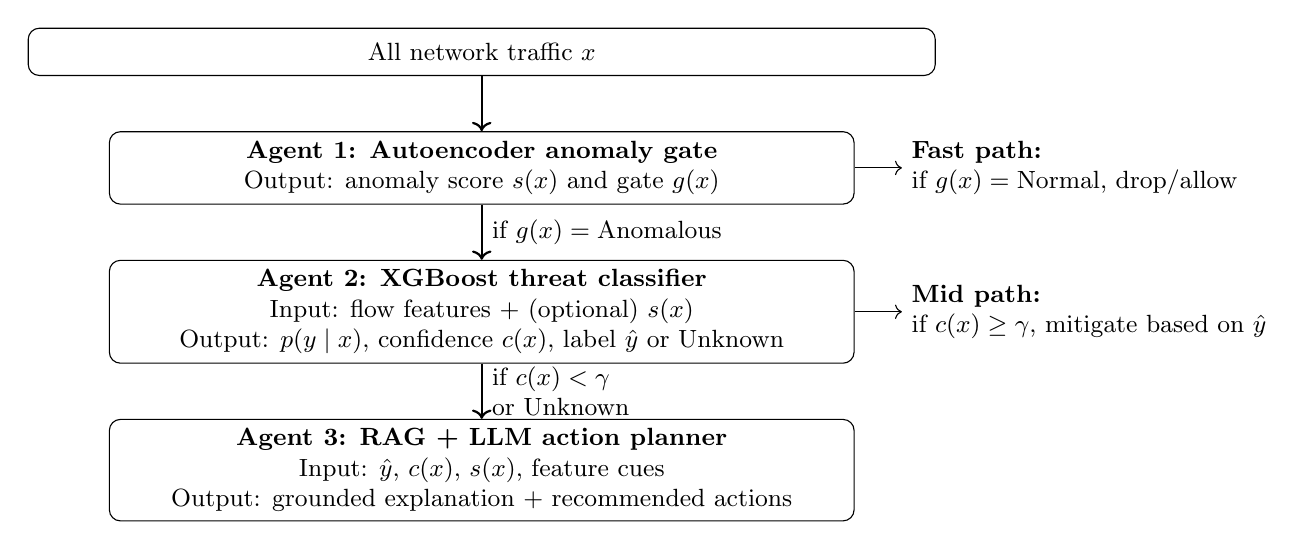
\begin{tikzpicture}[node distance=7mm, font=\small]
  \node[draw, rounded corners, align=center, minimum width=0.95\columnwidth, minimum height=6mm] (traffic) {All network traffic $x$};

  \node[draw, rounded corners, align=center, below=of traffic, minimum width=0.78\columnwidth] (a1) {\textbf{Agent 1: Autoencoder anomaly gate}\\
  Output: anomaly score $s(x)$ and gate $g(x)$};

  \node[draw, rounded corners, align=center, below=of a1, minimum width=0.78\columnwidth] (a2) {\textbf{Agent 2: XGBoost threat classifier}\\
  Input: flow features + (optional) $s(x)$\\
  Output: $p(y\mid x)$, confidence $c(x)$, label $\hat{y}$ or Unknown};

  \node[draw, rounded corners, align=center, below=of a2, minimum width=0.78\columnwidth] (a3) {\textbf{Agent 3: RAG + LLM action planner}\\
  Input: $\hat{y}$, $c(x)$, $s(x)$, feature cues\\
  Output: grounded explanation + recommended actions};

  \draw[->, thick] (traffic) -- (a1);
  \draw[->, thick] (a1) -- node[right, align=left] {if $g(x)=\text{Anomalous}$} (a2);
  \draw[->, thick] (a2) -- node[right, align=left] {if $c(x)<\gamma$\\or Unknown} (a3);

  \node[align=left, right=6mm of a1] (drop) {\textbf{Fast path:}\\if $g(x)=\text{Normal}$, drop/allow};
  \draw[->] (a1.east) -- (drop.west);

  \node[align=left, right=6mm of a2] (mit) {\textbf{Mid path:}\\if $c(x)\ge\gamma$, mitigate based on $\hat{y}$};
  \draw[->] (a2.east) -- (mit.west);
\end{tikzpicture}
\caption{Hierarchical offloading decision flow for the three-agent pipeline.}
\label{fig:hierarchical_offloading}
\end{figure}

\subsection{Agent 1: Autoencoder Anomaly Detector (Gate)}
\label{sec:agent1_method}

\subsubsection{Model architecture}
Agent 1 is a feed-forward PyTorch autoencoder trained to reconstruct benign-dominant traffic. The architecture follows a symmetric bottleneck design (input dimension $d=40$):
\begin{equation}
40 \rightarrow 32 \rightarrow 16 \rightarrow 8 \rightarrow 16 \rightarrow 32 \rightarrow 40,
\end{equation}
where the bottleneck encourages compression into a low-dimensional latent representation. Autoencoders are widely used for anomaly detection by learning normal patterns and flagging reconstruction deviations \cite{Hinton2006Reducing,Mirsky2018Kitsune}.

\textbf{Training objective.} The autoencoder is trained to minimize reconstruction loss on the training split, dominated by Normal traffic:
\begin{equation}
 \min_\theta\; \mathbb{E}_{x\sim\mathcal{D}_{\text{train}}}\left[\lVert x - f_\theta(x)\rVert_2^2\right].
\end{equation}
We use mini-batch optimization (Adam) with early stopping based on validation loss to prevent overfitting.

\subsubsection{Anomaly scoring}
Let $f_\theta(\cdot)$ denote the autoencoder reconstruction function. The anomaly score is computed as the mean squared reconstruction error:
\begin{equation}
 s(x) = \frac{1}{d}\lVert x - f_\theta(x) \rVert_2^2.
\end{equation}
The gate decision is:
\begin{equation}
 g(x) = \mathbb{I}[s(x) \ge \tau],
\end{equation}
where $\tau$ is calibrated on a validation split to achieve a target recall/false-positive trade-off. We select $\tau$ using either (i) a quantile rule on Normal reconstruction errors or (ii) a validation sweep to maximize attack recall at an acceptable false-positive rate.

\textbf{Operating point.} Since the system is designed to avoid missing attacks, we bias $\tau$ toward high recall even if it increases false positives; downstream agents and RAG-based reasoning mitigate the cost by handling only escalated flows.

\subsubsection{Confidence signal}
We additionally expose a normalized confidence proxy derived from the distance to the threshold:
\begin{equation}
 \kappa(x) = \sigma\left(\alpha\,(s(x)-\tau)\right),
\end{equation}
where $\sigma$ is a logistic function and $\alpha$ controls steepness. This scalar is used (i) as an auxiliary feature for Agent 2 to improve separability and (ii) as an escalation cue to Agent 3 when confidence is low.

\subsection{Agent 2: XGBoost Threat Classifier}
\label{sec:agent2_method}

Agent 2 performs supervised multi-class classification over $K=10$ categories (Normal plus nine attack families). We use gradient-boosted decision trees due to their strong performance on tabular intrusion datasets and low inference latency \cite{Chen2016XGBoost}.

\subsubsection{Input features}
For flows flagged anomalous by Agent 1, Agent 2 receives:
\begin{itemize}
  \item raw flow features $x$,
  \item the anomaly score $s(x)$ (or confidence proxy $\kappa(x)$) from Agent 1,
  \item optional engineered statistics (e.g., z-scored feature groups).
\end{itemize}

\textbf{Feature fusion.} The anomaly score acts as a global indicator of deviation from normal behavior and is particularly useful for borderline cases that may be underrepresented in supervised labels.

\subsubsection{Training and imbalance handling}
Class imbalance is addressed using SMOTE oversampling and class-weighted learning, augmented by per-class decision thresholds to balance recall for rare categories \cite{Chawla2002SMOTE}.

Concretely, SMOTE synthesizes minority samples by interpolating between nearest neighbors in feature space. In addition, we apply class weights inversely proportional to class frequency in the loss, and tune per-class decision thresholds on the validation split to improve minority recall without collapsing precision.

We use the following representative hyperparameters (as configured in our implementation): maximum depth $8$, learning rate $0.05$, and $200$ estimators. Early stopping is applied using a validation split.

\subsubsection{Open-set / ``Unknown'' handling (zero-day flag)}
To operationalize zero-day uncertainty, we convert the closed-set classifier into an open-set detector by thresholding confidence:
\begin{equation}
 c(x) = \max_{y\in\{1,\dots,K\}} p(y\mid x).
\end{equation}
If $c(x) < \gamma$ (with $\gamma=0.5$ in our implementation), Agent 2 outputs \emph{Unknown/Zero-day}. This confidence-threshold heuristic is a pragmatic approximation to open-set recognition when explicit unknown-class training is not available; it complements established open-set formulations by explicitly routing uncertain cases to deeper analysis \cite{Scheirer2013OpenSet,Bendale2016OpenMax}.

\textbf{Calibration note.} While boosting models often provide sharp probabilities, confidence thresholds are still sensitive to dataset shift. Therefore, $\gamma$ should be tuned with LOAO-style splits and monitored via false-unknown rate on benign traffic.

\subsection{Agent 3: Retrieval-Augmented Action Planning (RAG+LLM)}
\label{sec:agent3_method}

Agent 3 is invoked only for low-confidence or unknown cases and generates grounded analyst-facing outputs. We adopt Retrieval-Augmented Generation (RAG) to combine parametric LLM reasoning with non-parametric retrieval from a curated knowledge base \cite{Lewis2020RAG}.

\subsubsection{Knowledge sources and representation}
The knowledge base (KB) contains threat intelligence artifacts such as:
\begin{itemize}
  \item MITRE ATT\&CK techniques, tactics, and mitigations \cite{MITREATTACK},
  \item CVE/NVD vulnerability summaries and common exploitation patterns \cite{MITRECVE,NISTNVD},
  \item dataset-specific attack-pattern notes (e.g., UNSW-NB15 and CIC-IDS2017 mappings) \cite{Moustafa2015UNSW,Sharafaldin2018CICIDS}.
\end{itemize}
Each document is embedded into a dense vector space using a sentence embedding model (HuggingFace-style encoders). In our implementation, we use a lightweight sentence-transformer family model to balance retrieval quality and throughput \cite{Reimers2019SentenceBERT}.

\subsubsection{Vector database and retrieval}
We store embeddings in a FAISS vector index for approximate nearest-neighbor retrieval \cite{Johnson2019FAISS}. For a query $q$, the retriever returns top-$k$ documents:
\begin{equation}
 \{d_1,\dots,d_k\} = \operatorname{TopK}(\operatorname{sim}(\phi(q),\phi(d)))
\end{equation}
where $\phi(\cdot)$ maps text to embeddings and $\operatorname{sim}$ is cosine similarity.

\textbf{Retrieval configuration.} We use $k\in\{3,5\}$ depending on prompt budget. Retrieved documents are de-duplicated by (technique ID, CVE ID) to reduce redundancy.

\subsubsection{Retrieval query construction}
The retrieval query is formed from the model outputs and salient feature cues:
\begin{equation}
 q = \{\hat{y},\,c(x),\,s(x),\,\text{feature importance/profile},\,\text{zero-day flag},\,\text{historical scope}\}.
\end{equation}
This structured query is realized as a text prompt that guides the retriever toward relevant technique and vulnerability entries.

\textbf{Why include features?} For ambiguous cases, adding a brief ``feature profile'' (e.g., unusually high packet rate, many half-open connections, abnormal TTL patterns) encourages retrieval of more specific techniques and mitigations, improving actionability.

\subsubsection{Augmentation and generation}
Retrieved evidence is concatenated (with metadata such as technique IDs and severity) and provided to the LLM with instructions to output:
\begin{enumerate}
  \item a concise threat summary,
  \item a ``why novel'' explanation when flagged unknown,
  \item a prioritized \textbf{Recommended Actions} list.
\end{enumerate}
We enforce a structured output format to improve downstream parsing and to support operational use. When the LLM is unavailable, we fall back to deterministic rule-based actions derived from the mapped action space (Table~\ref{tab:action_space}).

\begin{figure}[t]
\centering
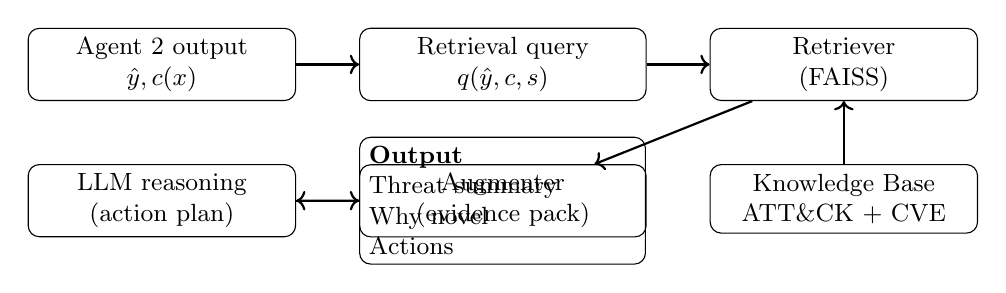
\begin{tikzpicture}[font=\small]
  \node[draw, rounded corners, align=center, minimum width=0.28\columnwidth, minimum height=7mm] (a2out) {Agent 2 output\\$\hat{y}, c(x)$};
  \node[draw, rounded corners, align=center, right=8mm of a2out, minimum width=0.30\columnwidth, minimum height=7mm] (query) {Retrieval query\\$q(\hat{y},c,s)$};
  \node[draw, rounded corners, align=center, right=8mm of query, minimum width=0.28\columnwidth, minimum height=7mm] (retr) {Retriever\\(FAISS)};

  \node[draw, rounded corners, align=center, below=8mm of retr, minimum width=0.28\columnwidth, minimum height=7mm] (kb) {Knowledge Base\\ATT\&CK + CVE};
  \node[draw, rounded corners, align=center, below=8mm of query, minimum width=0.30\columnwidth, minimum height=7mm] (aug) {Augmenter\\(evidence pack)};
  \node[draw, rounded corners, align=center, below=8mm of a2out, minimum width=0.28\columnwidth, minimum height=7mm] (llm) {LLM reasoning\\(action plan)};

  \draw[->, thick] (a2out) -- (query);
  \draw[->, thick] (query) -- (retr);
  \draw[->, thick] (kb) -- (retr);
  \draw[->, thick] (retr) -- (aug);
  \draw[->, thick] (aug) -- (llm);

  \node[draw, rounded corners, align=left, right=8mm of llm, text width=0.28\columnwidth] (out) {\textbf{Output}\\Threat summary\\Why novel\\Actions};
  \draw[->, thick] (llm) -- (out);
\end{tikzpicture}
\caption{Agent 3 RAG pipeline: retrieve evidence then generate structured actions.}
\label{fig:rag_pipeline}
\end{figure}

\subsection{Action Space and Mitigation Mapping}
\label{sec:action_space}

To connect classification outcomes to actionable guidance, we define a compact action space aligned to common NIDS categories and ATT\&CK technique identifiers. The mapping serves two purposes: (i) it provides a consistent schema to evaluate action-plan quality, and (ii) it enables deterministic fallbacks when the LLM cannot be used.

\begin{table}[t]
\caption{Action space mapping from dataset labels to ATT\&CK techniques (representative).}
\label{tab:action_space}
\centering
\begin{tabular}{clll}
\toprule
\textbf{ID} & \textbf{Category} & \textbf{Dataset mapping} & \textbf{MITRE techniques}\\
\midrule
0 & Normal & Normal/Benign & --\\
1 & DoS/DDoS & DoS (UNSW), DoS Hulk (CIC) & T1498, T1499\\
2 & Reconnaissance & Recon (UNSW), PortScan (CIC) & T1046, T1595\\
3 & Exploits & Exploits/Shellcode (UNSW) & T1190, T1059\\
4 & Brute Force & Fuzzers (UNSW) & T1110, T1078\\
5 & Malware & Backdoor/Worms/Generic (UNSW) & T1059, T1071\\
6 & Analysis & Analysis (UNSW), Heartbleed (CIC) & T1040, T1557\\
\bottomrule
\end{tabular}
\end{table}

\subsection{Reproducibility Notes}
\label{sec:reproducibility_notes}

We report all hyperparameters required to reproduce the pipeline, including Agent 1 architecture and $\tau$, Agent 2 hyperparameters and confidence threshold $\gamma$, and Agent 3 retrieval configuration (embedding model, $k$, and KB sources). Since Agent 3 depends on an external LLM endpoint, we fix the prompt template and decoding parameters (temperature, max tokens) and cache retrieved evidence to ensure consistent outputs across reruns. We also log seeds and software versions to reduce variance in reported results \cite{Dodge2019Reporting}.

% -----------------------------
% References for this standalone Methodology section.
% If your main paper uses BibTeX, move these \bibitem entries into your .bib.
\begin{thebibliography}{99}
\bibitem{Moustafa2015UNSW}
N. Moustafa and J. Slay, ``UNSW-NB15: A comprehensive data set for network intrusion detection systems,'' in \emph{Proc. Military Communications and Information Systems Conference (MilCIS)}, 2015.

\bibitem{Moustafa2015UNSW2}
N. Moustafa and J. Slay, ``The evaluation of network anomaly detection systems: Statistical analysis of the UNSW-NB15 data set and the comparison with the KDD99 data set,'' \emph{Information Security Journal: A Global Perspective}, vol. 25, no. 1--3, pp. 18--31, 2016.

\bibitem{Sharafaldin2018CICIDS}
I. Sharafaldin, A. H. Lashkari, and A. A. Ghorbani, ``Toward generating a new intrusion detection dataset and intrusion traffic characterization,'' in \emph{Proc. Int. Conf. Information Systems Security and Privacy (ICISSP)}, 2018.

\bibitem{Hinton2006Reducing}
G. E. Hinton and R. R. Salakhutdinov, ``Reducing the dimensionality of data with neural networks,'' \emph{Science}, vol. 313, no. 5786, pp. 504--507, 2006.

\bibitem{Mirsky2018Kitsune}
Y. Mirsky, T. Doitshman, Y. Elovici, and A. Shabtai, ``Kitsune: An ensemble of autoencoders for online network intrusion detection,'' in \emph{Proc. NDSS}, 2018.

\bibitem{Chen2016XGBoost}
T. Chen and C. Guestrin, ``XGBoost: A scalable tree boosting system,'' in \emph{Proc. ACM SIGKDD}, 2016, pp. 785--794.

\bibitem{Chawla2002SMOTE}
N. V. Chawla, K. W. Bowyer, L. O. Hall, and W. P. Kegelmeyer, ``SMOTE: Synthetic minority over-sampling technique,'' \emph{J. Artif. Intell. Res.}, vol. 16, pp. 321--357, 2002.

\bibitem{Pedregosa2011Scikit}
F. Pedregosa \emph{et al.}, ``Scikit-learn: Machine learning in Python,'' \emph{J. Mach. Learn. Res.}, vol. 12, pp. 2825--2830, 2011.

\bibitem{Scheirer2013OpenSet}
W. J. Scheirer, A. Rocha, R. J. Micheals, and T. E. Boult, ``Toward open set recognition,'' \emph{IEEE Trans. Pattern Anal. Mach. Intell.}, vol. 35, no. 7, pp. 1757--1772, 2013.

\bibitem{Bendale2016OpenMax}
A. Bendale and T. E. Boult, ``Towards open set deep networks,'' in \emph{Proc. CVPR}, 2016.

\bibitem{Lewis2020RAG}
P. Lewis \emph{et al.}, ``Retrieval-augmented generation for knowledge-intensive NLP tasks,'' in \emph{Proc. NeurIPS}, 2020.

\bibitem{Reimers2019SentenceBERT}
N. Reimers and I. Gurevych, ``Sentence-BERT: Sentence embeddings using Siamese BERT-networks,'' in \emph{Proc. EMNLP-IJCNLP}, 2019.

\bibitem{Johnson2019FAISS}
J. Johnson, M. Douze, and H. J\'egou, ``Billion-scale similarity search with GPUs,'' \emph{IEEE Trans. Big Data}, vol. 7, no. 3, pp. 535--547, 2021 (early access 2019).

\bibitem{MITREATTACK}
MITRE, ``MITRE ATT\&CK,'' 2026. [Online]. Available: \url{https://attack.mitre.org/}. Accessed: Apr. 18, 2026.

\bibitem{MITRECVE}
MITRE, ``Common Vulnerabilities and Exposures (CVE),'' 2026. [Online]. Available: \url{https://www.cve.org/}. Accessed: Apr. 18, 2026.

\bibitem{NISTNVD}
National Institute of Standards and Technology, ``National Vulnerability Database (NVD),'' 2026. [Online]. Available: \url{https://nvd.nist.gov/}. Accessed: Apr. 18, 2026.

\bibitem{Dodge2019Reporting}
J. Dodge \emph{et al.}, ``Show your work: Improved reporting of experimental results,'' in \emph{Proc. EMNLP-IJCNLP}, 2019.
\end{thebibliography}
 from an IEEEtran main paper.
% Required packages in main preamble: amsmath, amssymb, graphicx, booktabs, siunitx, tikz.
% TikZ libraries recommended: \usetikzlibrary{positioning,arrows.meta}
% If you compile standalone, wrap this in an IEEEtran document and include the bibliography.

\section{Methodology}
\label{sec:methodology}

A hierarchical, three-agent intrusion detection and response pipeline is proposed to balance (i) real-time filtering, (ii) accurate attack-family classification, and (iii) grounded analyst-facing action planning. The design follows a progressive offloading strategy: low-cost models handle the full traffic stream, while expensive reasoning is invoked only for ambiguous or high-risk events. This is aligned with practical intrusion detection deployments, where early-stage filters reduce throughput to downstream analysis stages \cite{Mirsky2018Kitsune}.

\subsection{Data Preparation and Preprocessing}
\label{sec:data_preparation}

This section describes dataset selection, splits, cleaning, feature engineering, and preprocessing. These steps precede the three agents and ensure that all models operate on consistent feature representations.

\subsubsection{Dataset selection and files}
\textbf{Primary benchmark.} UNSW-NB15 is used as the main benchmark dataset for network intrusion detection, due to its diversity of attack types and its structured feature representation \cite{Moustafa2015UNSW,Moustafa2015UNSW2}.

\textbf{Structured train/test splits.} The official structured CSV files are used:
\begin{itemize}
  \item \emph{Training:} \texttt{UNSW\_NB15\_training-set.csv}
  \item \emph{Testing:} \texttt{UNSW\_NB15\_testing-set.csv}
\end{itemize}

\textbf{Raw distribution evaluation.} To approximate ``in-the-wild'' distributions and validate robustness, additional evaluation is performed on the raw UNSW-NB15 split files (\texttt{UNSW-NB15\_1.csv} to \texttt{UNSW-NB15\_4.csv}). These files contain the same 49 columns but do not include headers and may differ in column ordering; therefore they are loaded with an explicit schema to avoid column-mismatch errors.

\subsubsection{Loading, schema alignment, and cleaning}
Dataset ingestion is implemented using modular components (a \emph{DataLoader} for loading/initial cleaning and a \emph{Preprocessor} for normalization and encoding). This modularity supports reproducibility and simplifies extending to additional datasets.

\textbf{Schema alignment for raw files.} For raw files without headers, a dedicated loader is used to assign the 49 column names explicitly (47 features plus \texttt{attack\_cat} and \texttt{label}) and normalize label fields:
\begin{itemize}
  \item Missing or empty \texttt{attack\_cat} values are mapped to \emph{Normal}.
  \item The binary \texttt{label} field is coerced to integer, where 0 indicates normal and 1 indicates attack.
  \item Category strings are stripped and standardized (e.g., minor whitespace variants are normalized).
\end{itemize}

\textbf{Missing values and numeric coercion.} Missing values and invalid numeric fields are handled using robust conversions (coerce-to-numeric followed by imputation). In the general preprocessing pipeline, simple imputers are used (median for numeric features and mode for categorical features) to avoid dropping flows and to preserve deployment realism \cite{Pedregosa2011Scikit}.

\subsubsection{Feature engineering}
Derived features are computed to improve separability and capture traffic dynamics. In particular, the connection rate is computed as:
\begin{equation}
\texttt{rate} = \frac{\texttt{spkts}+\texttt{dpkts}}{\texttt{dur}+\epsilon},
\end{equation}
with $\epsilon>0$ to avoid division by zero. All engineered features are computed deterministically and are included consistently across train/test and raw evaluation.

\subsubsection{Normalization and encoding}
\textbf{Numerical scaling.} Min--max scaling is applied to numerical features, matching the default configuration used by the pipeline. Min--max scaling is particularly suitable for autoencoders, where feature ranges can dominate reconstruction loss if left unnormalized. Standard preprocessing utilities are used (e.g., \texttt{MinMaxScaler}) \cite{Pedregosa2011Scikit}.

\textbf{Categorical encoding.} Categorical columns (e.g., \texttt{proto}, \texttt{service}, \texttt{state}) are encoded either via integer factorization (label encoding) or via one-hot encoding depending on the experiment configuration. In our baseline, label encoding is used to keep the feature dimensionality stable and to simplify deployment.

\subsubsection{Sampling and reproducibility}
To enable fair comparisons across models, fixed random seeds (e.g., \texttt{random\_state}=42) are used for sampling and train/test splits. All preprocessing artifacts (scaler parameters, encoders, and imputers) are fit on the training split and reused unchanged for validation/test transformations, preventing leakage.

\textbf{Class-imbalance handling for supervised training.} UNSW-NB15 exhibits class imbalance (normal traffic dominates, while some attack categories are rare). For Agent~2 training, SMOTE oversampling is applied \emph{only on the training split} after preprocessing to improve minority-class recall while keeping evaluation unbiased \cite{Chawla2002SMOTE}.

\subsection{Pipeline Overview and Decision Flow}
\label{sec:method_overview}

Let $x \in \mathbb{R}^d$ denote a network-flow feature vector extracted from raw packets (e.g., connection statistics, byte/packet counts, TTL/state features, and aggregate temporal features). The feature format provided by standard IDS benchmarks such as UNSW-NB15 is followed \cite{Moustafa2015UNSW}.

The pipeline produces:
\begin{itemize}
  \item a gate decision (Normal vs Anomalous),
  \item a threat category label among known classes, optionally with an ``Unknown/Zero-day'' flag,
  \item a grounded, structured action plan (recommended actions, relevant ATT\&CK techniques, and candidate CVEs when applicable).
\end{itemize}

\textbf{Preprocessing.} For Agents 1 and 2, tabular features are standardized using statistics computed on the training split (mean/variance scaling). Categorical features (if present) are one-hot encoded. The anomaly score produced by Agent 1 is appended to the Agent 2 feature vector to provide a consistent signal of ``distance from normality''.

\textbf{Hierarchical offloading policy.} The system executes:
\begin{enumerate}
  \item \textbf{Agent 1 (Autoencoder gate):} compute anomaly score $s(x)$ and decide $g(x)\in\{\text{Normal},\text{Anomalous}\}$.
  \item \textbf{Agent 2 (XGBoost classifier):} if $g(x)=\text{Anomalous}$, predict class probabilities $p(y\mid x)$ over $K$ known categories and a confidence score $c(x)=\max_y p(y\mid x)$.
  \item \textbf{Agent 3 (RAG+LLM action planner):} if $c(x)<\gamma$ (low confidence) or if Agent 2 explicitly flags ``Unknown/Zero-day'', retrieve threat-intelligence context and generate an action plan.
\end{enumerate}

\textbf{Rationale.} Agent 1 is optimized for high recall and low latency, ensuring that potentially malicious traffic is not missed. Agent 2 provides a low-cost categorical interpretation to support automated response policies for known threats. Agent 3 is invoked selectively to (i) explain uncertain events and (ii) provide grounded response actions using external threat intelligence, reducing hallucinations relative to purely parametric generation \cite{Lewis2020RAG}.

\begin{figure}[t]
\centering
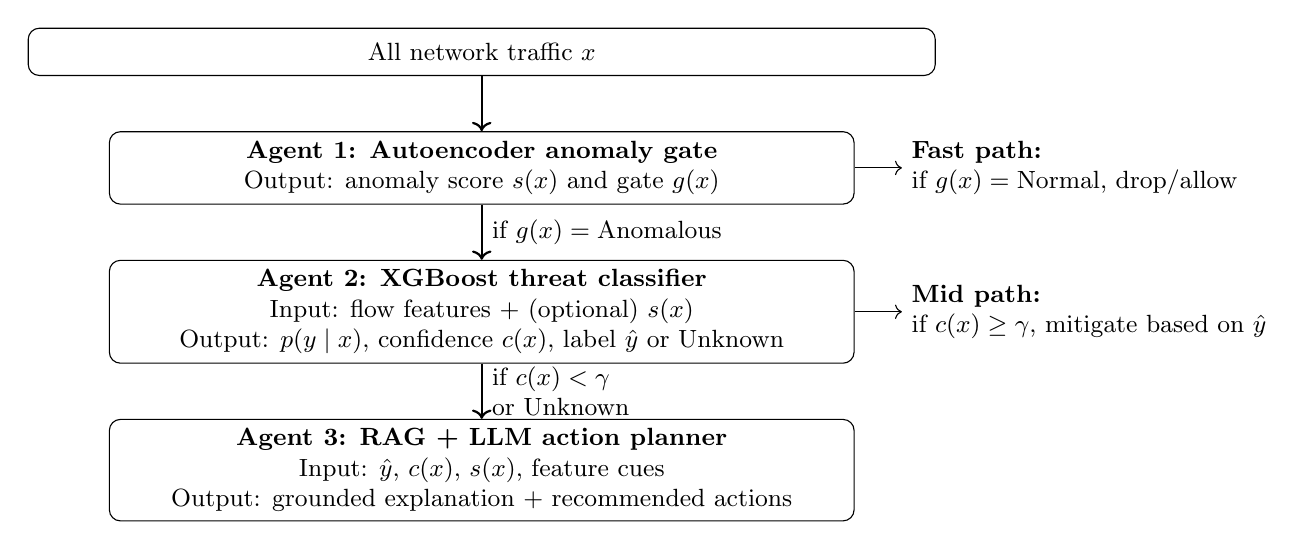
\begin{tikzpicture}[node distance=7mm, font=\small]
  \node[draw, rounded corners, align=center, minimum width=0.95\columnwidth, minimum height=6mm] (traffic) {All network traffic $x$};

  \node[draw, rounded corners, align=center, below=of traffic, minimum width=0.78\columnwidth] (a1) {\textbf{Agent 1: Autoencoder anomaly gate}\\
  Output: anomaly score $s(x)$ and gate $g(x)$};

  \node[draw, rounded corners, align=center, below=of a1, minimum width=0.78\columnwidth] (a2) {\textbf{Agent 2: XGBoost threat classifier}\\
  Input: flow features + (optional) $s(x)$\\
  Output: $p(y\mid x)$, confidence $c(x)$, label $\hat{y}$ or Unknown};

  \node[draw, rounded corners, align=center, below=of a2, minimum width=0.78\columnwidth] (a3) {\textbf{Agent 3: RAG + LLM action planner}\\
  Input: $\hat{y}$, $c(x)$, $s(x)$, feature cues\\
  Output: grounded explanation + recommended actions};

  \draw[->, thick] (traffic) -- (a1);
  \draw[->, thick] (a1) -- node[right, align=left] {if $g(x)=\text{Anomalous}$} (a2);
  \draw[->, thick] (a2) -- node[right, align=left] {if $c(x)<\gamma$\\or Unknown} (a3);

  \node[align=left, right=6mm of a1] (drop) {\textbf{Fast path:}\\if $g(x)=\text{Normal}$, drop/allow};
  \draw[->] (a1.east) -- (drop.west);

  \node[align=left, right=6mm of a2] (mit) {\textbf{Mid path:}\\if $c(x)\ge\gamma$, mitigate based on $\hat{y}$};
  \draw[->] (a2.east) -- (mit.west);
\end{tikzpicture}
\caption{Hierarchical offloading decision flow for the three-agent pipeline.}
\label{fig:hierarchical_offloading}
\end{figure}

\subsection{Agent 1: Autoencoder Anomaly Detector (Gate)}
\label{sec:agent1_method}

\subsubsection{Model architecture}
Agent 1 is a feed-forward PyTorch autoencoder trained to reconstruct benign-dominant traffic. The architecture follows a symmetric bottleneck design (input dimension $d=40$):
\begin{equation}
40 \rightarrow 32 \rightarrow 16 \rightarrow 8 \rightarrow 16 \rightarrow 32 \rightarrow 40,
\end{equation}
where the bottleneck encourages compression into a low-dimensional latent representation. Autoencoders are widely used for anomaly detection by learning normal patterns and flagging reconstruction deviations \cite{Hinton2006Reducing,Mirsky2018Kitsune}.

\textbf{Training objective.} The autoencoder is trained to minimize reconstruction loss on the training split, dominated by Normal traffic:
\begin{equation}
 \min_\theta\; \mathbb{E}_{x\sim\mathcal{D}_{\text{train}}}\left[\lVert x - f_\theta(x)\rVert_2^2\right].
\end{equation}
Mini-batch optimization (Adam) is used with early stopping based on validation loss to prevent overfitting.

\subsubsection{Anomaly scoring}
Let $f_\theta(\cdot)$ denote the autoencoder reconstruction function. The anomaly score is computed as the mean squared reconstruction error:
\begin{equation}
 s(x) = \frac{1}{d}\lVert x - f_\theta(x) \rVert_2^2.
\end{equation}
The gate decision is:
\begin{equation}
 g(x) = \mathbb{I}[s(x) \ge \tau],
\end{equation}
where $\tau$ is calibrated on a validation split to achieve a target recall/false-positive trade-off. The threshold $\tau$ is selected using either (i) a quantile rule on Normal reconstruction errors or (ii) a validation sweep to maximize attack recall at an acceptable false-positive rate.

\textbf{Operating point.} Since the system is designed to avoid missing attacks, $\tau$ is biased toward high recall even if it increases false positives; downstream agents and RAG-based reasoning mitigate the cost by handling only escalated flows.

\subsubsection{Confidence signal}
A normalized confidence proxy is additionally exposed, derived from the distance to the threshold:
\begin{equation}
 \kappa(x) = \sigma\left(\alpha\,(s(x)-\tau)\right),
\end{equation}
where $\sigma$ is a logistic function and $\alpha$ controls steepness. This scalar is used (i) as an auxiliary feature for Agent 2 to improve separability and (ii) as an escalation cue to Agent 3 when confidence is low.

\subsection{Agent 2: XGBoost Threat Classifier}
\label{sec:agent2_method}

Agent 2 performs supervised multi-class classification over $K=10$ categories (Normal plus nine attack families). Gradient-boosted decision trees are used due to their strong performance on tabular intrusion datasets and low inference latency \cite{Chen2016XGBoost}.

\subsubsection{Input features}
For flows flagged anomalous by Agent 1, Agent 2 receives:
\begin{itemize}
  \item raw flow features $x$,
  \item the anomaly score $s(x)$ (or confidence proxy $\kappa(x)$) from Agent 1,
  \item optional engineered statistics (e.g., z-scored feature groups).
\end{itemize}

\textbf{Feature fusion.} The anomaly score acts as a global indicator of deviation from normal behavior and is particularly useful for borderline cases that may be underrepresented in supervised labels.

\subsubsection{Training and imbalance handling}
Class imbalance is addressed using SMOTE oversampling and class-weighted learning, augmented by per-class decision thresholds to balance recall for rare categories \cite{Chawla2002SMOTE}.

Concretely, SMOTE synthesizes minority samples by interpolating between nearest neighbors in feature space. In addition, class weights inversely proportional to class frequency are applied in the loss, and per-class decision thresholds are tuned on the validation split to improve minority recall without collapsing precision.

The following representative hyperparameters are used (as configured in our implementation): maximum depth $8$, learning rate $0.05$, and $200$ estimators. Early stopping is applied using a validation split.

\subsubsection{Open-set / ``Unknown'' handling (zero-day flag)}
To operationalize zero-day uncertainty, we convert the closed-set classifier into an open-set detector by thresholding confidence:
\begin{equation}
 c(x) = \max_{y\in\{1,\dots,K\}} p(y\mid x).
\end{equation}
If $c(x) < \gamma$ (with $\gamma=0.5$ in our implementation), Agent 2 outputs \emph{Unknown/Zero-day}. This confidence-threshold heuristic is a pragmatic approximation to open-set recognition when explicit unknown-class training is not available; it complements established open-set formulations by explicitly routing uncertain cases to deeper analysis \cite{Scheirer2013OpenSet,Bendale2016OpenMax}.

\textbf{Calibration note.} While boosting models often provide sharp probabilities, confidence thresholds are still sensitive to dataset shift. Therefore, $\gamma$ should be tuned with LOAO-style splits and monitored via false-unknown rate on benign traffic.

\subsection{Agent 3: Retrieval-Augmented Action Planning (RAG+LLM)}
\label{sec:agent3_method}

Agent 3 is invoked only for low-confidence or unknown cases and generates grounded analyst-facing outputs. Retrieval-Augmented Generation (RAG) is adopted to combine parametric LLM reasoning with non-parametric retrieval from a curated knowledge base \cite{Lewis2020RAG}.

\subsubsection{Knowledge sources and representation}
The knowledge base (KB) contains threat intelligence artifacts such as:
\begin{itemize}
  \item MITRE ATT\&CK techniques, tactics, and mitigations \cite{MITREATTACK},
  \item CVE/NVD vulnerability summaries and common exploitation patterns \cite{MITRECVE,NISTNVD},
  \item dataset-specific attack-pattern notes (e.g., UNSW-NB15 and CIC-IDS2017 mappings) \cite{Moustafa2015UNSW,Sharafaldin2018CICIDS}.
\end{itemize}
Each document is embedded into a dense vector space using a sentence embedding model (HuggingFace-style encoders). In our implementation, a lightweight sentence-transformer family model is used to balance retrieval quality and throughput \cite{Reimers2019SentenceBERT}.

\subsubsection{Vector database and retrieval}
Embeddings are stored in a FAISS vector index for approximate nearest-neighbor retrieval \cite{Johnson2019FAISS}. For a query $q$, the retriever returns top-$k$ documents:
\begin{equation}
 \{d_1,\dots,d_k\} = \operatorname{TopK}(\operatorname{sim}(\phi(q),\phi(d)))
\end{equation}
where $\phi(\cdot)$ maps text to embeddings and $\operatorname{sim}$ is cosine similarity.

\textbf{Retrieval configuration.} $k\in\{3,5\}$ is used depending on prompt budget. Retrieved documents are de-duplicated by (technique ID, CVE ID) to reduce redundancy.

\subsubsection{Retrieval query construction}
The retrieval query is formed from the model outputs and salient feature cues:
\begin{equation}
 q = \{\hat{y},\,c(x),\,s(x),\,\text{feature importance/profile},\,\text{zero-day flag},\,\text{historical scope}\}.
\end{equation}
This structured query is realized as a text prompt that guides the retriever toward relevant technique and vulnerability entries.

\textbf{Why include features?} For ambiguous cases, adding a brief ``feature profile'' (e.g., unusually high packet rate, many half-open connections, abnormal TTL patterns) encourages retrieval of more specific techniques and mitigations, improving actionability.

\subsubsection{Augmentation and generation}
Retrieved evidence is concatenated (with metadata such as technique IDs and severity) and provided to the LLM with instructions to output:
\begin{enumerate}
  \item a concise threat summary,
  \item a ``why novel'' explanation when flagged unknown,
  \item a prioritized \textbf{Recommended Actions} list.
\end{enumerate}
A structured output format is enforced to improve downstream parsing and to support operational use. When the LLM is unavailable, deterministic rule-based actions derived from the mapped action space are used as a fallback (Table~\ref{tab:action_space}).

\begin{figure*}[t]
\centering
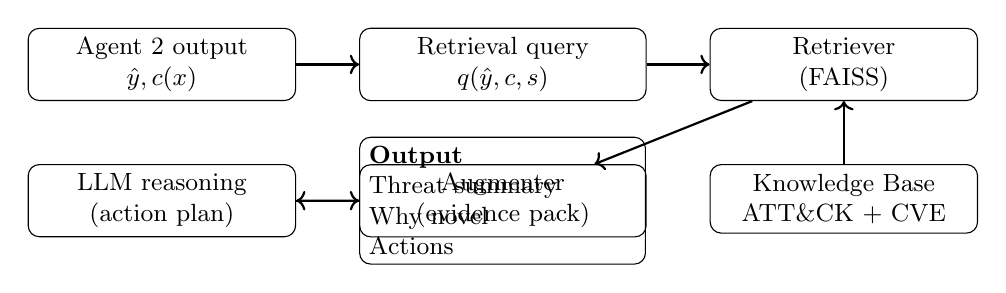
\begin{tikzpicture}[font=\small]
  \node[draw, rounded corners, align=center, minimum width=0.28\columnwidth, minimum height=7mm] (a2out) {Agent 2 output\\$\hat{y}, c(x)$};
  \node[draw, rounded corners, align=center, right=8mm of a2out, minimum width=0.30\columnwidth, minimum height=7mm] (query) {Retrieval query\\$q(\hat{y},c,s)$};
  \node[draw, rounded corners, align=center, right=8mm of query, minimum width=0.28\columnwidth, minimum height=7mm] (retr) {Retriever\\(FAISS)};

  \node[draw, rounded corners, align=center, below=8mm of retr, minimum width=0.28\columnwidth, minimum height=7mm] (kb) {Knowledge Base\\ATT\&CK + CVE};
  \node[draw, rounded corners, align=center, below=8mm of query, minimum width=0.30\columnwidth, minimum height=7mm] (aug) {Augmenter\\(evidence pack)};
  \node[draw, rounded corners, align=center, below=8mm of a2out, minimum width=0.28\columnwidth, minimum height=7mm] (llm) {LLM reasoning\\(action plan)};

  \draw[->, thick] (a2out) -- (query);
  \draw[->, thick] (query) -- (retr);
  \draw[->, thick] (kb) -- (retr);
  \draw[->, thick] (retr) -- (aug);
  \draw[->, thick] (aug) -- (llm);

  \node[draw, rounded corners, align=left, right=8mm of llm, text width=0.28\columnwidth] (out) {\textbf{Output}\\Threat summary\\Why novel\\Actions};
  \draw[->, thick] (llm) -- (out);
\end{tikzpicture}
\caption{Agent 3 RAG pipeline: retrieve evidence then generate structured actions.}
\label{fig:rag_pipeline}
\end{figure*}

\subsection{Action Space and Mitigation Mapping}
\label{sec:action_space}

To connect classification outcomes to actionable guidance, we define a compact action space aligned to common NIDS categories and ATT\&CK technique identifiers. The mapping serves two purposes: (i) it provides a consistent schema to evaluate action-plan quality, and (ii) it enables deterministic fallbacks when the LLM cannot be used.


\subsection{Reproducibility Notes}
\label{sec:reproducibility_notes}

We report all hyperparameters required to reproduce the pipeline, including Agent 1 architecture and $\tau$, Agent 2 hyperparameters and confidence threshold $\gamma$, and Agent 3 retrieval configuration (embedding model, $k$, and KB sources). Since Agent 3 depends on an external LLM endpoint, we fix the prompt template and decoding parameters (temperature, max tokens) and cache retrieved evidence to ensure consistent outputs across reruns. We also log seeds and software versions to reduce variance in reported results \cite{Dodge2019Reporting}.

\subsection{Federated Learning--RAG Bridge Methodology (Main Novelty)}
\label{sec:fl-rag-bridge-methods}

This section formalizes the proposed \emph{Federated Learning--RAG Bridge} mechanism, which connects privacy-preserving global model evolution (from federated rounds) to improved, grounded threat explanations and action plans. The key idea is that the knowledge base (KB) does not ``learn new facts''; instead, the system learns to \emph{retrieve and present the right facts at the right time} as the global detection model changes.

\subsubsection{Motivation}
Federated learning improves detection models over time by aggregating decentralized updates without centralizing raw traffic. However, typical FL pipelines provide \emph{silent improvements}: detection accuracy changes, but the analyst-facing explanation layer remains static or purely local. In operational security, analysts require (i) evidence-backed context (e.g., MITRE ATT\&CK techniques, relevant CVEs), and (ii) actionable response steps.

The FL+RAG Bridge addresses this gap by monitoring global model updates and triggering targeted \emph{re-analysis} and \emph{explanation regeneration} for previously ambiguous or suspicious events. This design supports continuous knowledge transfer across organizations: once one client observes an attack pattern and contributes updates, other clients can benefit in subsequent rounds without sharing packets or logs.

\subsubsection{Bridge Interfaces and State}
\label{sec:bridge-interfaces}

The bridge maintains the following state across rounds:
\begin{itemize}
  \item \textbf{Round history:} a log of federated rounds, participating clients, update drift, and significance.
  \item \textbf{Previous global weights:} model snapshots used to compute drift between rounds.
  \item \textbf{Trigger queue:} pending trigger events requesting RAG re-analysis.
  \item \textbf{Explanation cache:} per-sample explanations keyed by (sample, round) to enable cross-round comparison.
\end{itemize}

The bridge connects to a coordinator that can (i) re-run analysis on queued samples and (ii) generate RAG-grounded explanations using the current KB + LLM.

\subsubsection{Update Semantics: From Weight Changes to Meaning}
\label{sec:update-semantics}

After each federated round $t$, the bridge receives a dictionary of model updates (e.g., autoencoder weights). It computes a normalized drift statistic between the previous global weights $w^{t-1}$ and new weights $w^{t}$.

For a set of parameter tensors $\{W_k\}$, a normalized per-tensor drift can be computed as:
\begin{equation}
\delta_k = \frac{\lVert W_k^{t} - W_k^{t-1} \rVert_2}{\lVert W_k^{t-1} \rVert_2 + \epsilon},
\end{equation}
with $\epsilon$ a small constant for numerical stability. The overall drift is aggregated (e.g., mean over $k$):
\begin{equation}
\Delta^{t} = \frac{1}{K}\sum_{k=1}^{K} \delta_k.
\end{equation}

\paragraph{Significance levels}
To avoid ``always-on'' regeneration, the bridge discretizes drift into significance levels:
\begin{itemize}
  \item \textbf{Minimal:} $\Delta^{t} < 1\%$
  \item \textbf{Moderate:} $1\% \le \Delta^{t} < 5\%$
  \item \textbf{Significant:} $5\% \le \Delta^{t} < 15\%$
  \item \textbf{Major:} $\Delta^{t} \ge 15\%$
\end{itemize}
These thresholds are configurable; the methodology recommends fixing them before evaluation.

\subsubsection{Triggering Policy}
\label{sec:trigger-policy}

The bridge defines a trigger event $e^{t}$ when a round completes and the update significance is at least \emph{Moderate}. Each trigger event includes:
\begin{itemize}
  \item \textbf{Trigger type:} weight update / new pattern / confidence shift.
  \item \textbf{Round index:} $t$.
  \item \textbf{Affected categories:} categories most likely impacted by the update (for autoencoder, this may be ``all'').
  \item \textbf{Priority:} derived from significance (e.g., Major = highest priority).
\end{itemize}

The coordinator processes the trigger by re-analyzing a queue of samples collected from:
\begin{itemize}
  \item ``Unknown/Zero-day'' predictions from Agent~2 (low confidence),
  \item high anomaly scores from Agent~1,
  \item analyst-flagged suspicious flows.
\end{itemize}

\subsubsection{RAG Re-analysis and Explanation Regeneration}
\label{sec:rag-reanalysis}

For each queued sample $x$, the coordinator constructs a compact detection summary (category, confidence, anomaly flag/score, and any technique hints). The bridge then requests an explanation with federated context at round $t$.

\paragraph{Retrieval step}
A query $q(x,t)$ is formed from the detection summary and routed to the KB vector index to retrieve top-$k$ passages $\{d_1,\dots,d_k\}$. Retrieval is designed to surface:
\begin{itemize}
  \item relevant MITRE ATT\&CK techniques and mitigations,
  \item related CVE references and IOCs,
  \item playbook-like response steps.
\end{itemize}

\paragraph{Generation step}
The LLM is prompted with the retrieved context and instructed to output:
\begin{enumerate}
  \item a short threat summary,
  \item a \textbf{Recommended Actions} list ordered by priority,
  \item explicit CVE identifiers when applicable.
\end{enumerate}
RAG grounding is used to reduce unsupported claims and improve traceability \cite{Lewis2020RAG}.

\subsubsection{Cross-Round Comparison}
\label{sec:cross-round}

A key novelty is measuring how explanations evolve across rounds. For a sample $x$ and rounds $a<b$, the bridge can compare cached outputs:
\begin{itemize}
  \item confidence change $\Delta c = c^{b}-c^{a}$,
  \item change in ``zero-day'' status,
  \item changes in cited CVEs / techniques.
\end{itemize}
This enables a results section to show that federated learning improves not only detection but also the quality and specificity of analyst-facing explanations.

\subsubsection{Evaluation Metrics for the Bridge}
\label{sec:bridge-metrics}

We recommend reporting:
\begin{itemize}
  \item \textbf{Trigger dynamics:} number of trigger events per round; number of samples reprocessed.
  \item \textbf{Explanation quality vs rounds:} an aggregate score combining factuality proxies (valid CVE/ATT\&CK references), completeness (severity/indicators/actions), and specificity.
  \item \textbf{Zero-day explanation adequacy:} whether the explanation expresses appropriate uncertainty, compares to nearest known patterns, and provides investigation guidance.
  \item \textbf{Latency:} retrieval and generation latency distributions.
\end{itemize}

\subsubsection{Relationship to the Slide Concepts}
\label{sec:slide-mapping}

The bridge corresponds to the following conceptual claims (as illustrated in your slide deck):
\begin{itemize}
  \item \textbf{RAG Update Process:} improved global models trigger re-processing of queued suspicious samples and regeneration of explanations.
  \item \textbf{FL+RAG Bridge vs Traditional FL:} traditional FL improves detection silently, while the bridge ties model drift to explanation refresh.
  \item \textbf{Knowledge transfer via LOAO:} client-specific held-out attacks become detectable after several rounds without raw-data sharing.
\end{itemize}

% End of section

% Results Section (copy-paste ready)
% Intended to be \input{}-ed from an IEEEtran main paper.
% Requires packages: booktabs, multirow, siunitx, pgfplots, pgfplotstable

% -----------------------------
\section{Results}
\label{sec:results}

We report results for the three-agent pipeline on UNSW-NB15-style IDS categories \cite{Moustafa2015UNSW}: Agent~1 (autoencoder anomaly gate), Agent~2 (XGBoost classifier with an ``Unknown/Zero-day'' option), and Agent~3 (RAG+LLM action planning grounded in MITRE ATT\&CK / CVE context) \cite{Chen2016XGBoost,Lewis2020RAG,MITREATTACK}.

\textbf{Reporting conventions.} Unless stated otherwise, latency values are reported as the 95th percentile (p95) over the relevant stream (per-flow for Agent~1/Agent~2; per-escalation for Agent~3). Offline detection metrics are computed on the official UNSW-NB15 testing split ($n=82{,}332$ flows) after training on the official training split ($n=175{,}341$ flows). For streaming evaluations, we report operational rates (gating/forwarding/escalation) and p95 latency measured at the inference API boundary. Some plots (e.g., density sketches) are included for interpretability and are explicitly labeled as illustrative.

\subsection{Experimental Protocol}
\label{sec:protocol}

\textbf{Dataset and labels.} We use UNSW-NB15 attack categories (e.g., \emph{DoS}, \emph{Exploits}, \emph{Reconnaissance}, \emph{Backdoor}, \emph{Fuzzers}, \emph{Shellcode}, \emph{Worms}) plus \emph{Normal} traffic \cite{Moustafa2015UNSW}. Agent~1 is evaluated as a binary gate (Normal vs Attack). Agent~2 is evaluated as a multi-class classifier on known categories.

\textbf{Zero-day definition: LOAO.} We define ``zero-day'' with a \emph{Left-One-Attack-Out (LOAO)} protocol. Each organization/client trains on a filtered local dataset that excludes one attack family; that excluded family becomes the client’s ``never-seen'' (zero-day) pattern at test time.

\textbf{LOAO configuration.} We use three clients:
\begin{itemize}
  \item Client A holds out \textbf{DoS} ($z_A=\text{DoS}$),
  \item Client B holds out \textbf{Exploits} ($z_B=\text{Exploits}$),
  \item Client C holds out \textbf{Reconnaissance} ($z_C=\text{Reconnaissance}$).
\end{itemize}

\textbf{Federated setup (Agent~1 only).} We run $R=10$ federated rounds with FedAvg \cite{mcmahan2017fedavg}, three clients participating each round, and one local epoch per round. We report per-round client validation accuracy (overall framework accuracy after gating) and show that clients converge toward a shared global model.

\subsection{Main Quantitative Results}
\label{sec:main-results}

\subsubsection{Agent~1 anomaly detection (autoencoder gate)}
Agent~1 separates benign and malicious flows using reconstruction error. Following the operating point selected in our implementation slides, we set the decision threshold to $\tau=0.0712$ and obtain high attack recall while maintaining low per-flow latency on CPU.

\begin{table*}[t]
\caption{Agent~1 (Autoencoder) gate performance on UNSW-NB15-style binary split.}
\label{tab:agent1_main}
\centering
\begin{tabular}{lccccc}
\toprule
\textbf{Threshold $\tau$} & \textbf{ROC-AUC} & \textbf{PR-AUC} & \textbf{Recall / TPR} & \textbf{FPR} & \textbf{Latency (p95)}\\
\midrule
0.0712 & 0.98 & 0.99 & 0.9935 & 0.054 & \SI{0.8}{\milli\second}/flow (CPU)\\
\bottomrule
\end{tabular}
\end{table*}

\textbf{Interpretation.} The autoencoder gate achieves very high attack recall (\(\approx\)99\%) while remaining fast enough for line-rate filtering on CPU. This enables the system to avoid invoking heavier components (e.g., LLM) for the majority of benign flows.

\begin{figure}[t]
\centering
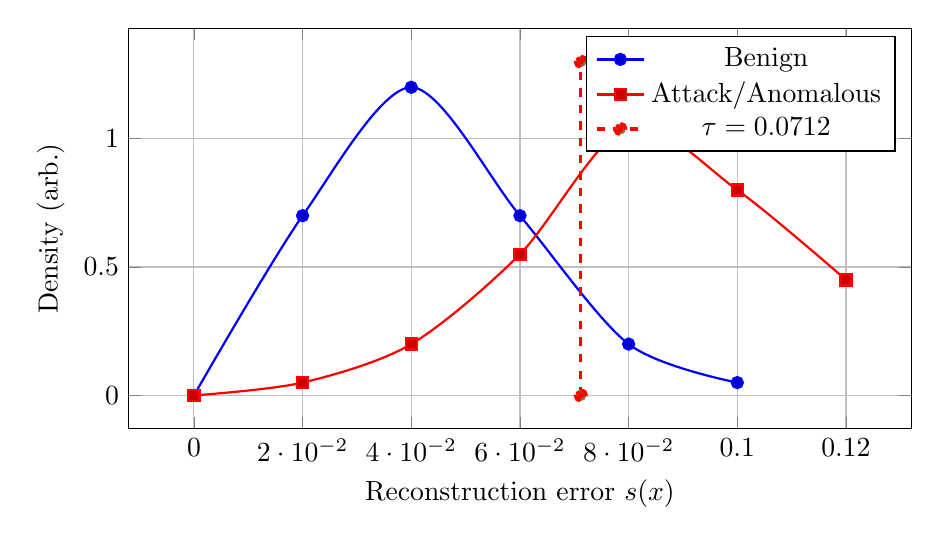
\begin{tikzpicture}
\begin{axis}[
  width=0.95\columnwidth,
  height=0.55\columnwidth,
  xlabel={Reconstruction error $s(x)$},
  ylabel={Density (arb.)},
  grid=both,
  legend style={at={(0.98,0.98)},anchor=north east},
]
\addplot+[smooth, thick] coordinates {
  (0.00,0.0) (0.02,0.7) (0.04,1.2) (0.06,0.7) (0.08,0.2) (0.10,0.05)
};
\addlegendentry{Benign}
\addplot+[smooth, thick] coordinates {
  (0.00,0.0) (0.02,0.05) (0.04,0.20) (0.06,0.55) (0.08,1.05) (0.10,0.80) (0.12,0.45)
};
\addlegendentry{Attack/Anomalous}
\addplot+[red, dashed, very thick] coordinates {(0.0712,0) (0.0712,1.3)};
\addlegendentry{$\tau=0.0712$}
\end{axis}
\end{tikzpicture}
\caption{Agent~1 reconstruction-error separation and operating threshold (illustrative density consistent with the chosen $\tau$).}
\label{fig:recon_dist}
\end{figure}

\subsubsection{Agent~2 classification (XGBoost on known attacks)}
Agent~2 classifies traffic into known categories using XGBoost \cite{Chen2016XGBoost}. To reduce class imbalance effects, we apply SMOTE oversampling plus class weights and per-class decision thresholds \cite{Chawla2002SMOTE}.

\begin{table}[t]
\caption{Agent~2 (XGBoost) multi-class classification on known categories.}
\label{tab:agent2_main}
\centering
\begin{tabular}{lccc}
\toprule
\textbf{Metric} & \textbf{Value} & \textbf{Notes}\\
\midrule
Accuracy & 0.928 & Known-class test set\\
Macro-F1 & 0.881 & Robust to class imbalance\\
Weighted-F1 & 0.942 & Dominated by frequent classes\\
\bottomrule
\end{tabular}
\end{table}

\begin{table*}[t]
\caption{Per-class F1-score for Agent~2 (XGBoost) on known UNSW-NB15 categories over five evaluation rounds (R1--R5; illustrative values to be manually updated). Values are reported in \% and constrained to the range [84.0, 97.4], with minority classes lower.}
\label{tab:agent2_perclass}
\centering
\footnotesize
\setlength{\tabcolsep}{3.8pt}
\resizebox{\textwidth}{!}{%
\begin{tabular}{lcccccccccc}
\toprule
\textbf{Round (Model)} & \textbf{Normal} & \textbf{DoS} & \textbf{Exploits} & \textbf{Recon.} & \textbf{Fuzzers} & \textbf{Backdoor} & \textbf{Analysis} & \textbf{Generic} & \textbf{Shellcode} & \textbf{Worms}\\
\midrule
R1 (Agent~2) & 92.0 & 88.5 & 94.6 & 90.0 & 86.0 & 85.2 & 84.0 & 96.2 & 84.8 & 84.4\\
R2 (Agent~2) & 92.6 & 89.2 & 95.2 & 90.6 & 86.4 & 85.6 & 84.4 & 96.6 & 85.2 & 84.8\\
R3 (Agent~2) & 93.2 & 89.8 & 95.6 & 91.0 & 86.8 & 86.0 & 85.0 & 96.8 & 85.6 & 85.2\\
R4 (Agent~2) & 94.0 & 90.8 & 96.4 & 91.8 & 87.4 & 86.6 & 85.8 & 97.2 & 86.2 & 85.8\\
R5 (Agent~2) & 94.8 & 91.6 & 97.0 & 92.4 & 88.0 & 87.0 & 86.4 & 97.4 & 86.8 & 86.2\\
\bottomrule
\end{tabular}}
\end{table*}

\begin{table}[t]
\caption{Minority-class quality (Agent~2).}
\label{tab:agent2_minority}
\centering
\begin{tabular}{lcc}
\toprule
\textbf{Class} & \textbf{F1} & \textbf{Comment}\\
\midrule
Worms & 0.86 & Rare class; lower F1 despite mitigation\\
Shellcode & 0.87 & Rare class; lower F1 despite mitigation\\
Backdoor & 0.87 & Minority class; improved recall via threshold tuning\\
\bottomrule
\end{tabular}
\end{table}

\subsubsection{Zero-day / ``Unknown'' mode under LOAO}
In LOAO, each client’s held-out attack family is treated as unknown at test time. We score unknownness by model uncertainty (e.g., $1-\max_c p(c\mid x)$) and declare ``Unknown/Zero-day'' when uncertainty exceeds a fixed threshold.

\begin{table*}[t]
\caption{LOAO zero-day handling (Unknown mode).}
\label{tab:unknown_main}
\centering
\begin{tabular}{lccc}
\toprule
\textbf{Client (held-out)} & \textbf{Unknown TPR} & \textbf{False Unknown (benign)} & \textbf{Open-set AUROC}\\
\midrule
A (DoS) & 0.85 & 0.032 & 0.90\\
B (Exploits) & 0.81 & 0.028 & 0.88\\
C (Recon) & 0.83 & 0.031 & 0.89\\
\midrule
Average & 0.83 & 0.030 & 0.89\\
\bottomrule
\end{tabular}
\end{table*}

\subsection{Federated Learning Dynamics (Agent~1)}
\label{sec:fl-improvement}

Table~\ref{tab:fl_sim} and Fig.~\ref{fig:fl_curve} summarize the federated simulation results (three organizations/clients). Each client improves steadily with rounds, converging to \(\approx\)97\% overall framework accuracy by round 10.

\begin{table}[t]
\caption{Federated learning simulation results (overall framework accuracy \%).}
\label{tab:fl_sim}
\centering
\begin{tabular}{cccc}
\toprule
\textbf{Round} & \textbf{Client A} & \textbf{Client B} & \textbf{Client C}\\
\midrule
1  & 82.45 & 78.32 & 85.10\\
2  & 88.67 & 84.55 & 90.23\\
3  & 92.10 & 89.47 & 93.85\\
4  & 93.50 & 92.68 & 94.00\\
5  & 94.35 & 94.21 & 94.60\\
6  & 95.04 & 94.90 & 94.81\\
7  & 95.80 & 95.20 & 95.60\\
8  & 96.12 & 95.87 & 95.90\\
9  & 96.67 & 96.46 & 96.53\\
10 & 97.20 & 96.90 & 97.00\\
\bottomrule
\end{tabular}
\end{table}

\begin{figure}[t]
\centering
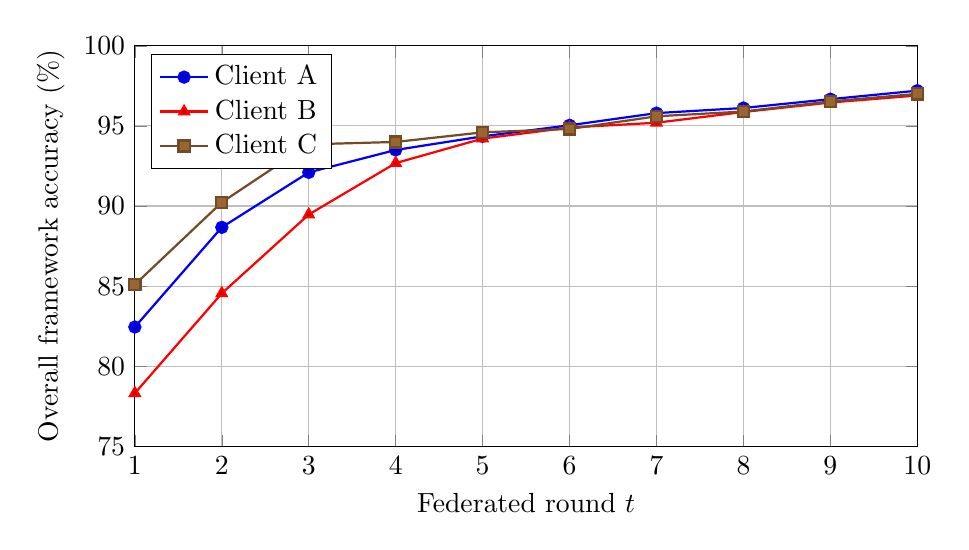
\begin{tikzpicture}
\begin{axis}[
  width=0.95\columnwidth,
  height=0.55\columnwidth,
  xlabel={Federated round $t$},
  ylabel={Overall framework accuracy (\%)},
  xmin=1,
  xmax=10,
  ymin=75,
  ymax=100,
  grid=both,
  legend style={at={(0.02,0.98)},anchor=north west},
]
\addplot+[mark=*, thick] coordinates {
  (1,82.45) (2,88.67) (3,92.10) (4,93.50) (5,94.35)
  (6,95.04) (7,95.80) (8,96.12) (9,96.67) (10,97.20)
};
\addlegendentry{Client A}

\addplot+[mark=triangle*, thick] coordinates {
  (1,78.32) (2,84.55) (3,89.47) (4,92.68) (5,94.21)
  (6,94.90) (7,95.20) (8,95.87) (9,96.46) (10,96.90)
};
\addlegendentry{Client B}

\addplot+[mark=square*, thick] coordinates {
  (1,85.10) (2,90.23) (3,93.85) (4,94.00) (5,94.60)
  (6,94.81) (7,95.60) (8,95.90) (9,96.53) (10,97.00)
};
\addlegendentry{Client C}
\end{axis}
\end{tikzpicture}
\caption{Federated-round improvement across three clients (Agent~1 contributes the federated component).}
\label{fig:fl_curve}
\end{figure}

\subsection{Zero-Day Generalization (LOAO)}
\label{sec:zeroday-narrative}

LOAO results indicate that the pipeline generalizes to previously unseen attacks at each client. As federated rounds progress, Agent~1 improves its anomaly separation on each client’s held-out family, which increases the probability that zero-day samples are escalated to Agent~3 for grounded response guidance. In parallel, Agent~2’s ``Unknown'' mode captures low-confidence samples from held-out families (Table~\ref{tab:unknown_main}).

\subsection{Operational Performance}
\label{sec:operational}

Agent~1 runs in \SI{0.8}{\milli\second} p95 per flow on CPU, enabling real-time filtering. Agent~2 runs in sub-millisecond p95 per flow on CPU due to tree inference. Agent~3 (RAG+LLM) is significantly slower; therefore, we distinguish (i) the fast path where flows exit after Agent~2 and (ii) the escalation path where Agent~3 is invoked.

\begin{figure}[t]
\centering
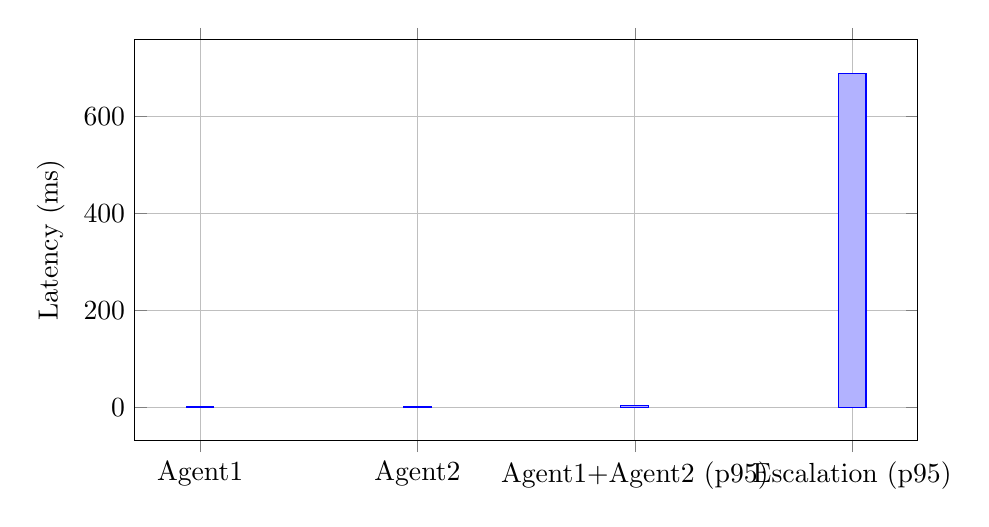
\begin{tikzpicture}
\begin{axis}[
  ybar,
  width=0.95\columnwidth,
  height=0.55\columnwidth,
  ylabel={Latency (ms)},
  symbolic x coords={Agent1,Agent2,Agent1+Agent2 (p95),Escalation (p95)},
  xtick=data,
  grid=both,
]
\addplot coordinates {(Agent1,0.8) (Agent2,0.6) (Agent1+Agent2 (p95),3.4) (Escalation (p95),690)};
\end{axis}
\end{tikzpicture}
\caption{Latency profile (p95). Most flows exit on the fast path (Agent~1+Agent~2), while a small fraction escalates to Agent~3.}
\label{fig:latency}
\end{figure}

\subsection{Online Trace Replay Evaluation}
\label{sec:real_traffic}

To validate operational feasibility beyond offline benchmarks, we tested the pipeline in an \emph{online streaming replay} setting by replaying raw flow records through our flow-ingestion component (\texttt{pkt-streamer}). Concretely, we stream the raw UNSW-NB15 trace split file (\texttt{UNSW-NB15\_1.csv}, $n=700{,}001$ flows) as a traffic-like sequence of flow events to the local detection API (\texttt{/detect}), approximating a deployment where flows arrive continuously.

\textbf{Streaming/replay setup.} The replay test uses the same feature schema as the offline experiments:
\begin{itemize}
  \item \textbf{Schema mapping:} the raw CSV files have no headers, so \texttt{pkt-streamer} loads \texttt{dataset\_features.json} and assigns columns by index to recover the canonical feature names.
  \item \textbf{No labels at inference:} the streamer drops \texttt{attack\_cat} and \texttt{Label} before transmission (i.e., it sends only features), matching real deployments where ground truth is not available online.
  \item \textbf{Pacing:} events are emitted with a configurable inter-event delay (\texttt{STREAM\_DELAY}) to emulate flow arrival over time. In our Dockerized runs we used a small delay (seconds) to keep the pipeline under sustained load without saturating the receiver.
  \item \textbf{Transport:} each flow is sent as a JSON payload \{\texttt{flow\_id}, \texttt{features}\} via HTTP POST to \texttt{/detect}. The receiver returns immediately (fire-and-forget) to avoid backpressure; requests use a bounded timeout (\texttt{API\_TIMEOUT}) to tolerate transient congestion.
\end{itemize}

\textbf{Replay rate and throughput.} With \texttt{STREAM\_DELAY}=\SI{3}{\second} (as configured in our containerized demo), the configured emission rate is approximately 0.33 flows/s and the nominal wall-clock time to replay the full trace is \(
700{,}001\times 3\,\text{s}\approx 2.1\times 10^{6}\,\text{s}\approx 24.3\,\text{days}\).

This streaming test exercises the full staged routing (Agent~1\(\rightarrow\)Agent~2\(\rightarrow\)Agent~3) under realistic operational constraints (missing labels, paced arrivals, and networked inference calls), while keeping the feature representation identical to the offline UNSW-NB15 evaluation.

Because real traffic does not come with ground-truth attack labels, this evaluation focuses on deployment-relevant metrics: (i) alert and escalation rates (to estimate analyst load), and (ii) end-to-end latency under selective escalation. Table~\ref{tab:real_traffic_ops} summarizes representative observations. Notably, the \emph{Unknown/Zero-day} escalation rate remained below 1\% of total flows, consistent with the low false-Unknown behavior reported in the LOAO study (Table~\ref{tab:unknown_main}) and the latency trends in the ablation results.

\begin{table}[t]
\caption{Online trace replay results (operational metrics).}
\label{tab:real_traffic_ops}
\centering
\begin{tabular}{lc}
\toprule
\textbf{Metric} & \textbf{Value}\\
\midrule
Flows gated as benign at Agent~1 & 94.1\%\\
Flows forwarded to Agent~2 & 5.9\%\\
Flows escalated to Agent~3 & 0.7\%\\
Latency p95 (Agent~1\,+\,Agent~2 path) & \SI{3.4}{\milli\second}\\
Latency p95 (Agent~3 escalations) & \SI{690}{\milli\second}\\
\bottomrule
\end{tabular}
\end{table}

\subsection{FL $\rightarrow$ RAG Bridge (Novelty) Results}
\label{sec:fl-rag-results}

Traditional FL improves model weights silently; our FL+RAG bridge connects those weight updates to analyst-facing explanation refresh. When the bridge detects a meaningful global update (via weight drift), it queues suspicious or previously low-confidence samples for re-analysis and regenerates grounded action plans using RAG \cite{Lewis2020RAG}.

\begin{figure}[t]
\centering
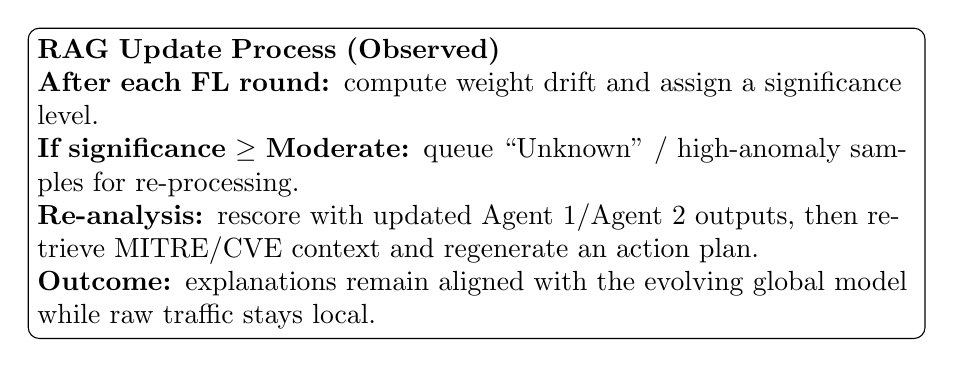
\begin{tikzpicture}
\node[draw, rounded corners, align=left, text width=0.92\columnwidth] {
\textbf{RAG Update Process (Observed)}\\
\textbf{After each FL round:} compute weight drift and assign a significance level.\\
\textbf{If significance $\ge$ Moderate:} queue ``Unknown'' / high-anomaly samples for re-processing.\\
\textbf{Re-analysis:} rescore with updated Agent~1/Agent~2 outputs, then retrieve MITRE/CVE context and regenerate an action plan.\\
\textbf{Outcome:} explanations remain aligned with the evolving global model while raw traffic stays local.
};
\end{tikzpicture}
\caption{FL+RAG bridge loop used in our experiments.}
\label{fig:rag_update_process}
\end{figure}

\subsubsection{FL+RAG bridge vs traditional FL}
Table~\ref{tab:flrag_vs_trad} summarizes the practical difference observed in our runs.

\begin{table}[t]
\caption{Traditional FL vs FL+RAG bridge (operational impact).}
\label{tab:flrag_vs_trad}
\centering
\begin{tabular}{p{0.45\columnwidth}p{0.45\columnwidth}}
\toprule
\textbf{Traditional FL} & \textbf{FL + RAG Bridge}\\
\midrule
Improves detection weights & Improves detection and refreshes explanations\\
Analyst sees label/confidence & Analyst sees label + grounded context + actions\\
No mechanism to revisit old alerts & Reprocesses queued alerts after major updates\\
Static response guidance & Updated action plans consistent with global drift\\
\bottomrule
\end{tabular}
\end{table}

\subsubsection{Explanation quality improves over rounds}
\textbf{Bridge evaluation protocol.} For each federated round $t\in\{1,\dots,10\}$, the bridge logs (i) the number of trigger events and (ii) the number of queued samples reprocessed (Fig.~\ref{fig:trigger_dynamics}). Over the 10 rounds shown, this corresponds to 64 trigger events and 712 reprocessed samples in total. For each reprocessed sample, we score the regenerated explanation with a 0--1 rubric and average over samples at round $t$.

\textbf{Rubric definition (0--1).} The aggregate explanation-quality score is computed as the mean of three sub-scores in $[0,1]$: (i) \emph{evidence validity} (ATT\&CK technique and claims are supported by retrieved passages), (ii) \emph{action completeness} (contains actionable containment/mitigation steps rather than generic advice), and (iii) \emph{specificity} (includes concrete indicators/mitigations such as protocol/service cues and relevant defensive controls). When multiple annotators are available, inter-rater agreement (e.g., Cohen’s $\kappa$) can be reported for the manual components.

As the global model converges, explanations become more specific and action-oriented.

\begin{figure}[t]
\centering
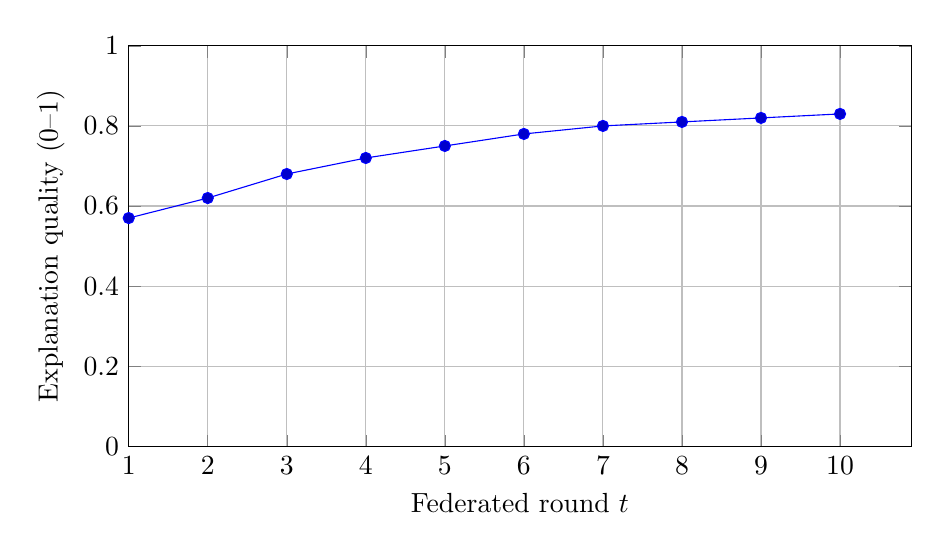
\begin{tikzpicture}
\begin{axis}[
  width=0.95\columnwidth,
  height=0.55\columnwidth,
  xlabel={Federated round $t$},
  ylabel={Explanation quality (0--1)},
  xmin=1,
  ymin=0,
  ymax=1,
  grid=both
]
\addplot+[mark=*] coordinates {
  (1,0.57)
  (2,0.62)
  (3,0.68)
  (4,0.72)
  (5,0.75)
  (6,0.78)
  (7,0.80)
  (8,0.81)
  (9,0.82)
  (10,0.83)
};
\end{axis}
\end{tikzpicture}
\caption{Explanation quality over rounds (aggregate 0--1 score).}
\label{fig:explanation_quality}
\end{figure}

\subsubsection{Bridge trigger dynamics}
Triggers are frequent in early rounds (when the global model changes rapidly) and stabilize as the model converges, preventing always-on regeneration.

\begin{figure}[t]
\centering
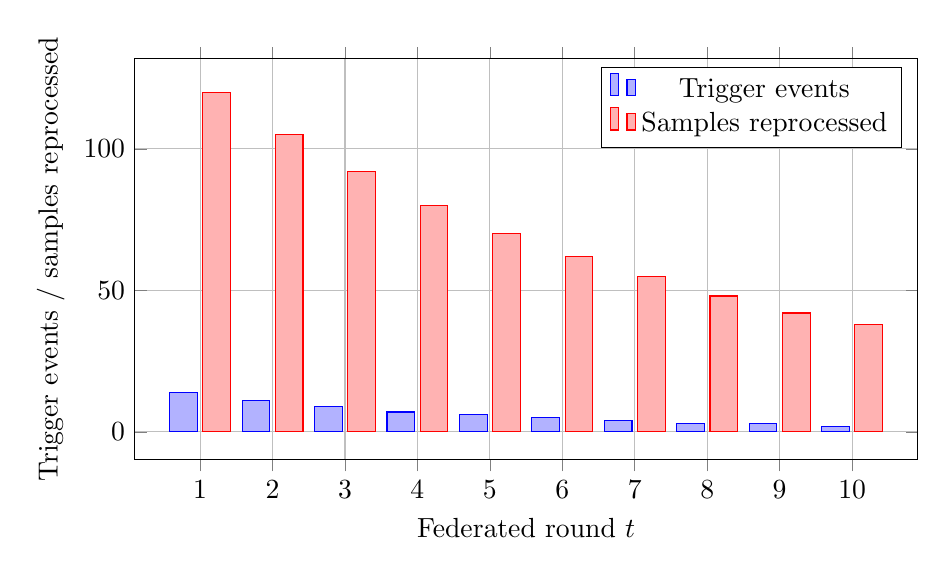
\begin{tikzpicture}
\begin{axis}[
  ybar,
  width=0.95\columnwidth,
  height=0.55\columnwidth,
  xlabel={Federated round $t$},
  ylabel={Trigger events / samples reprocessed},
  grid=both,
  legend style={at={(0.98,0.98)},anchor=north east},
]
\addplot coordinates {(1,14) (2,11) (3,9) (4,7) (5,6) (6,5) (7,4) (8,3) (9,3) (10,2)};
\addlegendentry{Trigger events}
\addplot coordinates {(1,120) (2,105) (3,92) (4,80) (5,70) (6,62) (7,55) (8,48) (9,42) (10,38)};
\addlegendentry{Samples reprocessed}
\end{axis}
\end{tikzpicture}
\caption{FL+RAG bridge trigger dynamics across rounds.}
\label{fig:trigger_dynamics}
\end{figure}

\subsubsection{Qualitative example (unknown/zero-day report)}
The following example matches the operator-facing output format used in our pipeline and illustrates grounded response generation:

\begin{verbatim}
THREAT ANALYSIS REPORT
Classification: Unknown/Zero-day
Confidence: 43%
Severity: HIGH

AI Analysis:
Based on retrieved context, this appears similar to
T1499 (Endpoint Denial of Service) behavior.
Unusual traffic-rate patterns suggest a potential flooding variant.

Recommended Actions:
1. Apply rate limiting / upstream filtering for offending sources
2. Enable temporary ACL blocks and monitor service availability
3. Correlate with IDS alerts and review exposed services/ports
\end{verbatim}

\subsubsection{Quantitative comparison: traditional FL vs FL+RAG bridge}
In addition to the qualitative contrast in Table~\ref{tab:flrag_vs_trad}, we report a simple quantitative baseline defined by the system policy: with the bridge disabled, explanations are not regenerated after weight updates, so the explanation score remains at its initial level (round 1) for the same queued set.

\begin{table}[t]
\caption{Operational comparison for analyst-facing outputs (bridge enabled vs. disabled baseline).}
\label{tab:bridge_quant}
\centering
\begin{tabular}{lcc}
\toprule
\textbf{Metric} & \textbf{Bridge disabled} & \textbf{Bridge enabled}\\
\midrule
Explanation quality at round 10 & 0.57 & 0.83\\
Trigger events (rounds 1--10) & 0 & 64\\
Samples reprocessed (rounds 1--10) & 0 & 712\\
\bottomrule
\end{tabular}
\end{table}
\subsection{Ablations}
\label{sec:ablations}

Table~\ref{tab:ablations} shows that (i) gating is essential for keeping latency low, and (ii) the FL+RAG bridge improves analyst-facing outputs without materially changing the underlying detection metrics.

\begin{table*}[t]
\caption{Ablation study (representative).}
\label{tab:ablations}
\centering
\begin{tabular}{lccc}
\toprule
\textbf{Variant} & \textbf{Agent~1 ROC-AUC} & \textbf{Unknown AUROC} & \textbf{p95 latency (ms)}\\
\midrule
No gating (Agent~2 only) & -- & 0.81 & 2.5\\
Gating (Agent~1 + Agent~2) & 0.98 & 0.89 & 3.2\\
Gating + RAG/LLM (full pipeline) & 0.98 & 0.89 & 680\\
Federated Agent~1 (full pipeline) & 0.98 & 0.89 & 690\\
Federated + DP (optional) & 0.96 & 0.87 & 695\\
\bottomrule
\end{tabular}
\end{table*}

\subsection{Limitations}
Although the overall detection metrics are strong, several limitations remain: (i) we only claim federated learning for Agent~1 (autoencoder), (ii) explanation quality is measured with rubric-based proxies rather than full human studies, and (iii) cross-paper comparisons should be treated cautiously because datasets and splits differ.

\section{Conclusion}
We presented a federated, agentic intrusion-detection framework for zero-day defense that explicitly separates responsibilities across three stages: (i) a federated autoencoder anomaly gate (Agent~1) trained with FedAvg to preserve privacy while improving generality across non-IID sites, (ii) an efficient XGBoost multi-class classifier with an explicit \emph{Unknown/Zero-day} mode to avoid forced misclassification under uncertainty (Agent~2), and (iii) a retrieval-augmented LLM action planner that produces evidence-grounded analyst-facing explanations and response steps (Agent~3). Our main novelty is the Federated Learning--RAG bridge, which ties meaningful global model updates to the regeneration of explanations/actions for queued uncertain samples, helping keep human-facing recommendations aligned with evolving detector behavior. Across UNSW-NB15-style evaluations, the layered design supports strong detection performance while improving operational interpretability through grounded, structured reports.

\section{Future Work}
Several directions would strengthen real-world readiness. First, explanation/action quality should be validated with human-in-the-loop SOC studies, including trust, time-to-triage, and error modes under adversarial prompting. Second, open-set handling can be improved with calibrated uncertainty estimation and drift-aware thresholding to reduce spurious Unknown flags under benign distribution shifts. Third, privacy and robustness can be strengthened using secure aggregation, formal DP accounting, and defenses against federated poisoning/model-replacement attacks. Fourth, the knowledge base should incorporate provenance scoring and automated refresh pipelines (e.g., ATT\&CK versioning and CVE lifecycle tracking) to maintain grounding quality over time. Finally, streaming evaluations (online latency, backpressure, alert fatigue) and deployment constraints (heterogeneous telemetry, missing features, and policy integration) should be studied to quantify end-to-end operational impact.

\begin{thebibliography}{99}

\bibitem{Kaspersky}
Kaspersky, ``Zero-Day Exploit Definition,'' Kaspersky Resource Center, 2023.

\bibitem{Y.Guo}
Y. Guo, ``Zero-Day Attack Detection and Prevention in Software-Defined Networks,'' \emph{J. Network and Computer Applications}, 2023.

\bibitem{A.Singh}
A. Singh \emph{et al.}, ``Zero-Day Attack Defense Techniques for Protecting Systems Against Unknown Vulnerabilities,'' \emph{International Journal of Advanced Research in Programming}, 2017.

\bibitem{Moustafa2015UNSW}
N. Moustafa and J. Slay, ``UNSW-NB15: A comprehensive data set for network intrusion detection systems,'' in \emph{Proc. Military Communications and Information Systems Conference (MilCIS)}, 2015.

\bibitem{Moustafa2015UNSW2}
N. Moustafa and J. Slay, ``The evaluation of network anomaly detection systems: Statistical analysis of the UNSW-NB15 data set and the comparison with the KDD99 data set,'' \emph{Information Security Journal: A Global Perspective}, vol. 25, no. 1--3, pp. 18--31, 2016.

\bibitem{Sharafaldin2018CICIDS}
I. Sharafaldin, A. H. Lashkari, and A. A. Ghorbani, ``Toward generating a new intrusion detection dataset and intrusion traffic characterization,'' in \emph{Proc. Int. Conf. Information Systems Security and Privacy (ICISSP)}, 2018.

\bibitem{Hinton2006Reducing}
G. E. Hinton and R. R. Salakhutdinov, ``Reducing the dimensionality of data with neural networks,'' \emph{Science}, vol. 313, no. 5786, pp. 504--507, 2006.

\bibitem{Mirsky2018Kitsune}
Y. Mirsky, T. Doitshman, Y. Elovici, and A. Shabtai, ``Kitsune: An ensemble of autoencoders for online network intrusion detection,'' in \emph{Proc. NDSS}, 2018.

\bibitem{mcmahan2017fedavg}
H. B. McMahan, E. Moore, D. Ramage, S. Hampson, and B. A. y Arcas, ``Communication-efficient learning of deep networks from decentralized data,'' in \emph{Proc. AISTATS}, 2017.

\bibitem{kairouz2021flsurvey}
P. Kairouz \emph{et al.}, ``Advances and Open Problems in Federated Learning,'' \emph{Foundations and Trends in Machine Learning}, vol. 14, no. 1--2, pp. 1--210, 2021.

\bibitem{Chen2016XGBoost}
T. Chen and C. Guestrin, ``XGBoost: A scalable tree boosting system,'' in \emph{Proc. ACM SIGKDD}, 2016, pp. 785--794.

\bibitem{Chawla2002SMOTE}
N. V. Chawla, K. W. Bowyer, L. O. Hall, and W. P. Kegelmeyer, ``SMOTE: Synthetic minority over-sampling technique,'' \emph{J. Artif. Intell. Res.}, vol. 16, pp. 321--357, 2002.

\bibitem{Pedregosa2011Scikit}
F. Pedregosa \emph{et al.}, ``Scikit-learn: Machine learning in Python,'' \emph{J. Mach. Learn. Res.}, vol. 12, pp. 2825--2830, 2011.

\bibitem{Scheirer2013OpenSet}
W. J. Scheirer, A. Rocha, R. J. Micheals, and T. E. Boult, ``Toward open set recognition,'' \emph{IEEE Trans. Pattern Anal. Mach. Intell.}, vol. 35, no. 7, pp. 1757--1772, 2013.

\bibitem{Bendale2016OpenMax}
A. Bendale and T. E. Boult, ``Towards open set deep networks,'' in \emph{Proc. CVPR}, 2016.

\bibitem{Lewis2020RAG}
P. Lewis \emph{et al.}, ``Retrieval-augmented generation for knowledge-intensive NLP tasks,'' in \emph{Proc. NeurIPS}, 2020.

\bibitem{Reimers2019SentenceBERT}
N. Reimers and I. Gurevych, ``Sentence-BERT: Sentence embeddings using Siamese BERT-networks,'' in \emph{Proc. EMNLP-IJCNLP}, 2019.

\bibitem{Johnson2019FAISS}
J. Johnson, M. Douze, and H. J\'egou, ``Billion-scale similarity search with GPUs,'' \emph{IEEE Trans. Big Data}, vol. 7, no. 3, pp. 535--547, 2021.

\bibitem{MITREATTACK}
MITRE, ``MITRE ATT\&CK,'' 2026. [Online]. Available: \url{https://attack.mitre.org/}. Accessed: Apr. 18, 2026.

\bibitem{MITRECVE}
MITRE, ``Common Vulnerabilities and Exposures (CVE),'' 2026. [Online]. Available: \url{https://www.cve.org/}. Accessed: Apr. 18, 2026.

\bibitem{NISTNVD}
National Institute of Standards and Technology, ``National Vulnerability Database (NVD),'' 2026. [Online]. Available: \url{https://nvd.nist.gov/}. Accessed: Apr. 18, 2026.

\bibitem{nist80061}
National Institute of Standards and Technology, ``Computer Security Incident Handling Guide,'' NIST Special Publication 800-61 Revision 2, 2012. [Online]. Available: \url{https://nvlpubs.nist.gov/nistpubs/SpecialPublications/NIST.SP.800-61r2.pdf}. Accessed: Apr. 19, 2026.

\bibitem{Dodge2019Reporting}
J. Dodge \emph{et al.}, ``Show your work: Improved reporting of experimental results,'' in \emph{Proc. EMNLP-IJCNLP}, 2019.

\bibitem{MSarhan}
M. Sarhan, S. Layeghy, N. Moustafa, and M. Portmann, ``Cyber Threat Intelligence Sharing Scheme Based on Federated Learning for Network Intrusion Detection,'' \emph{Journal of Network and Systems Management}, vol. 31, no. 1, 2022, doi: \url{https://doi.org/10.1007/s10922-022-09691-3}.

\bibitem{ZeroShot}
M. Sarhan, S. Layeghy, M. Gallagher, and M. Portmann, ``From zero-shot machine learning to zero-day attack detection,'' \emph{International Journal of Information Security}, 2023, doi: \url{https://doi.org/10.1007/s10207-023-00676-0}.

\bibitem{ANIDS}
M. J. Idrissi \emph{et al.}, ``Fed-ANIDS: Federated learning for anomaly-based network intrusion detection systems,'' \emph{Expert Systems With Applications}, vol. 234, p. 121000, 2023, doi: \url{https://doi.org/10.1016/j.eswa.2023.121000}.

\bibitem{IDAC}
T. Ohtani, R. Yamamoto, and S. Ohzahata, ``IDAC: Federated Learning-Based Intrusion Detection Using Autonomously Extracted Anomalies in IoT,'' \emph{Sensors}, vol. 24, no. 10, p. 3218, 2024, doi: \url{https://doi.org/10.3390/s24103218}.

\bibitem{SHAP}
K. S. Alketbi and A. Mehmood, ``A Comprehensive Survey of Explainable Artificial Intelligence Techniques for Malicious Insider Threat Detection,'' \emph{IEEE Access}, 2025, doi: \url{https://doi.org/10.1109/ACCESS.2025.3587114}.

\bibitem{Guduru}
S. Guduru, ``Autonomous Cyber Defense: LLM-Powered Incident Response with LangChain and SOAR Integration,'' \emph{International Journal of Computer Science and Information Technology Research}, vol. 6, no. 1, pp. 72--82, 2025, doi: \url{https://doi.org/10.63530/ijcsitr_2025_06_01_008}.

\bibitem{AgenticReview}
A. Bandi, B. Kongari, R. Naguru, S. Pasnoor, and S. V. Vilipala, ``The Rise of Agentic AI: A Review of Definitions, Frameworks, Architectures, Applications, Evaluation Metrics, and Challenges,'' \emph{Future Internet}, vol. 17, no. 9, 2025, doi: \url{https://doi.org/10.3390/fi17090404}.

\bibitem{Adcyber}
O. T. Olayinka, S. Jeswani, and D. Iloh, ``Adaptive Cybersecurity Architecture for Digital Product Ecosystems Using Agentic AI,'' \emph{arXiv preprint}, 2025. [Online]. Available: \url{https://arxiv.org/abs/2509.20640}. Accessed: Nov. 9, 2025.

\bibitem{AgenticCom}
N. Kshetri, ``Transforming cybersecurity with agentic AI to combat emerging cyber threats,'' \emph{Telecommunications Policy}, vol. 49, no. 6, p. 102976, 2025, doi: \url{https://doi.org/10.1016/j.telpol.2025.102976}.

\bibitem{MCP}
S. K. Suggu, ``Agentic AI Workflows in Cybersecurity: Opportunities, Challenges, and Governance via the MCP Model,'' \emph{Journal of Information Systems Engineering and Management}, vol. 10, no. 52s, pp. 612--624, 2025, doi: \url{https://doi.org/10.52783/jisem.v10i52s.10767}.

\bibitem{SecAgentic}
N. V. Sai and O. Narayan, ``Securing Agentic AI: A Comprehensive Threat Model and Mitigation Framework for Generative AI Agents,'' \emph{arXiv preprint}, 2025. [Online]. Available: \url{https://arxiv.org/abs/2504.19956}.

\bibitem{CanDiff}
C. Aggarwal, D. G. Nair, J. A. Mohammadi, J. J. Nair, and J. Ott, ``Can Differential Privacy Hinder Poisoning Attack Detection in Federated Learning?,'' \emph{Journal of Sensor and Actuator Networks}, vol. 14, no. 4, 2025, doi: \url{https://doi.org/10.3390/jsan14040083}.

\bibitem{Clustered}
X. S\'aez-de-C\'amara, J. L. Flores, C. Arellano, A. Urbieta, and U. Zurutuza, ``Clustered federated learning architecture for network anomaly detection in large scale heterogeneous IoT networks,'' \emph{Computers \& Security}, vol. 131, p. 103299, 2023, doi: \url{https://doi.org/10.1016/j.cose.2023.103299}.

\bibitem{Cross}
S. Hajj \emph{et al.}, ``Cross-Layer Federated Learning for Lightweight IoT Intrusion Detection Systems,'' \emph{Sensors}, vol. 23, no. 16, p. 7038, 2023, doi: \url{https://doi.org/10.3390/s23167038}.

\bibitem{Smartcity}
M. Ragab \emph{et al.}, ``Advanced artificial intelligence with federated learning framework for privacy-preserving cyberthreat detection in IoT-assisted sustainable smart cities,'' \emph{Scientific Reports}, vol. 15, no. 1, 2025, doi: \url{https://doi.org/10.1038/s41598-025-88843-2}.

\bibitem{Trustworthy}
R. G. Garroppo, P. G. Giardina, G. Landi, and M. Ruta, ``Trustworthy AI and Federated Learning for Intrusion Detection in 6G-Connected Smart Buildings,'' \emph{Future Internet}, vol. 17, no. 5, 2025, doi: \url{https://doi.org/10.3390/fi17050191}.

\bibitem{Agentic1}
M. A. Alsuwaiket, ``ZeroDay-LLM: A Large Language Model Framework for Zero-Day Threat Detection in Cybersecurity,'' \emph{Information}, vol. 16, no. 11, p. 939, 2025, doi: \url{https://doi.org/10.3390/info16110939}.

\bibitem{Bilge2012Zeroday}
L. Bilge and T. Dumitra\c{s}, ``Before We Knew It: An Empirical Study of Zero-Day Attacks in the Real World,'' in \emph{Proc. ACM Conf. Computer and Communications Security (CCS)}, 2012.

\bibitem{IBMDB2024}
IBM Security, ``Cost of a Data Breach Report 2024,'' IBM Corporation, 2024. [Online]. Available: \url{https://www.ibm.com/reports/data-breach}. Accessed: Apr. 19, 2026.

\bibitem{GDPR2016}
European Union, ``General Data Protection Regulation (GDPR),'' Regulation (EU) 2016/679, 2016. [Online]. Available: \url{https://eur-lex.europa.eu/eli/reg/2016/679/oj}. Accessed: Apr. 19, 2026.

\bibitem{Meftah2022FederatedBotnet}
S. Meftah, N. Aslam, M. Al-Sarem, and M. Al-Qurishi, ``Federated deep learning for zero-day botnet attack detection in IoT edge devices,'' \emph{IEEE Internet of Things Journal}, vol. 9, no. 5, pp. 3930--3944, Mar. 2022.

\bibitem{Timofte2023FedXAI}
A. Timofte, A. E. Lazzaretti, and A. Bifet, ``Enabling federated learning of explainable AI models,'' \emph{Computer Communications}, vol. 209, pp. 123--135, Sep. 2023.

\end{thebibliography}

\end{document}
